%%==============================================================================
%  Model exercise Numerical computation of CD/LP experiment (Mont Terri)
%  BV, 24/04/2019
%%==============================================================================
\section{Model Exercise 1-4 (10): CD/LP experiment (Mont Terri)}
\label{sec:mex10}
%------------------------------------------------------------------------------
\Authors{Bernhard Vowinckel, Gesa Ziefle, Jobst Ma\ss mann}
%------------------------------------------------------------------------------
\subsection{Motivation}
%%%%%%%%%%%%%%%%%%%%%%%%%%%%%%%%%%%%%%%%%%%%%%%%%%%%%%%%%%%%%%%%%%%%%%%%%%%%%%%%%%%%%%%%%%%%
Various areas of research like disopsal of nuclear radioactive waste, geothermal energy, and carbon capture and storage (CCS) among others deal with coupled hydraulic-mechanical as well as thermal and chemical processes in the underground. Finite element (FE) codes are a well established tool to strengthen the understanding of the related long-term effects. The German Federal Institute for Geosciences and Natural Resources (BGR) has gathered vast experience with the FE code OpenGeoSys (OGS-5 as described in \cite{kolditz2012})  to compute coupled  hydraulic-mechanical processes for example in the  Mont Terri Rock Laboratory (RL) in Switzerland. Within the project GeomInt (Geomechanical integrity of host and barrier rocks), the focus is on the investigation of the development of discontinuities such as cracks and fissures in claystone, crystalline and rock salt. The Helmholtz Centre for Environmental Research (UFZ) is developing an enhanced version of the FE code OGS-6 (as described in \cite{Naumov:2018}) which has an additional focus on the investigation of these effects.   The present report summarizes the results of a comparison between two simulations of the seasonally induced hydraulic desiccation carried out using OGS-5 (version from November 13th, 2017) and OGS-6 (version from December 7th, 2018), respectively. The comparison focuses on the implementation of the two model approaches: 1) Unsaturated one phase flow, based on the Richards approximation \cite{richards1931} (”Richards Flow”, RF) and 2) poro-elasticity coupled with Richards Flow following \cite{biot1941} (”Richards Mechanics”, RM). These models serve as a basis to extend OGS-6 further towards the
dynamics of discontinuities.

%%%%%%%%%%%%%%%%%%%%%%%%%%%%%%%%%%%%%%%%%%%%%%%%%%%%%%%%%%%%%%%%%%%%%%%%%%%%%%%%%%%%%%%%%%%%
\subsection{Problem statement}
%%%%%%%%%%%%%%%%%%%%%%%%%%%%%%%%%%%%%%%%%%%%%%%%%%%%%%%%%%%%%%%%%%%%%%%%%%%%%%%%%%%%%%%%%%%%
In the present study, we analyze an idealized niche that is located in the anticline of the Opalinus Clay formation of Mont Terri RL and has a width and height of 3.15 m and 3.3 m, respectively. The computational scenario is designed according to \cite{ziefle2018}, who successfully reproduced the coupled hydraulic-mechanical behavior of a niche in the tunnel system of the Mont Terri RL.   A cross-sectional view of the model of the niche is given in Figure \ref{fig:setup}. The clayey rock in the niche is uncovered, so that seasonal changes in humidity cause cyclic desiccation and saturation of the rock. The porous medium is subdivided into two material groups. Far away from the niche ($> 2$ m), the rock is undisturbed and reflects the properties of Opalinus clay (ID 1). Close to the niche, an excavation damaged zone (EDZ) is defined (ID 2). For the present study, two relevant processes can be identified. First, owing to the exposure of the niche to seasonal change in humidity, there will be a saturation/desaturation of the porous rock. This process can be analyzed by considering hydraulic effects (RF) only. Second, the changes in capillary pressure induce a stress redistribution. To analyze this problem, the coupled hydro-mechanical process (RM) needs to be considered.

%%%%%%%%%%%%%%%%%%%%%%%%%%%%%%%%%%%%%%%%%%%%%%%%%%%%%%%%%%%%%%%%%%%%%%%%%%%%%%%%%%%%%%%%%%%%
\subsection{Unsaturated one-phase flow using the Richards approximation ( "Richards Flow", RF)}\label{sec:RF}
\subsubsection{Model description}\label{sec:model_RF}
%%%%%%%%%%%%%%%%%%%%%%%%%%%%%%%%%%%%%%%%%%%%%%%%%%%%%%%%%%%%%%%%%%%%%%%%%%%%%%%%%%%%%%%%%%%%
The model "Richards Flow" (RF) is based on the classical Richards equation for unsaturated conditions in porous media flows \cite{richards1931}, which reads:
\begin{equation}\label{eq:richards}
\phi \rho_f \frac{\partial S}{\partial p_c}\frac{\partial p_c}{\partial t} + \nabla \cdot \left(\rho_f \frac{k_\text{rel}\textbf{k}}{\mu_f}(\nabla p_f-\rho_f \textbf{g})\right)= Q_f \qquad ,
\end{equation}
where $\phi$ is the porosity, $\rho_f$ the fluid density, $S$ the fluid saturation, $p_c$ the capillary pressure, $t$ the time, $k_\text{rel}$ the relative permeability, $\textbf{k}$ the intrinsic permeability, $\mu_f$ the dynamic viscosity of water, $p_f=-p_c$ the fluid pressure, $\textbf{g}$ the vector of gravitational acceleration, and $Q_f$ a source term. Note that this approximation neglects the change of gas pressure. Equation \eqref{eq:richards} is parametrized using the classical van Genuchten approach  \cite{vangenuchten1980} for the capillary pressure
\begin{equation}\label{eq:cap_p}
p_c = \max \left(p_d\left(S_\text{eff}^{-1/m}-1\right)^{1-m};p_{c,max}\right)
\end{equation}
and the relative permeability 
\begin{equation}\label{eq:k_rel}
k_\text{rel}=S_\text{eff}^{1/2}\left[1-\left(1-S_\text{eff}^{1-\beta}\right)^\beta\right]^2 \qquad ,
\end{equation}
respectively, where $p_d$ is the air entry pressure, $m$ and $\beta$ are fitting parameters reflecting the pore size distribution, $p_{c,max}$ is the maximum capillary pressure and 
\begin{equation}
S_\text{eff}=\frac{S-S_r}{S_{max}-S_r}
\end{equation}
is the effective saturation. Here, $S_r$ and $S_\text{max}$ are the residual and maximum fluid saturation, respectively.

Parameters were taken from the simulations carried out by \cite{ziefle2018}:
\begin{tabbing} 
Fluid density 		\hspace{4cm} \= $\rho_f=1000 \text{ kg/m}^3$	\\
Dynamic viscosity 	\>				$\mu_f= 1\cdot 10^{-3} \,  \text{Pa s}$\\
Porosity 			\> 				$\phi=0.16$ 					\\
Air entry pressure	\>				$p_d = 2 \cdot 10^{7} \, \text{Pa}$\\
Maximum capillary pressure \> 		$p_{c,max} = 1 \cdot 10^9 \, \text{Pa}$\\
Parameter for capillary pressure   \>	$m = 0.41176$\\
Parameter for relative permeability\> 	$\beta = 0.5$ \\
Residual fluid saturation \>			$S_r = 0.0$ \\
Maximum fluid saturation \> 			$S_\text{max}=1.0$ \\
Gravitational acceleration \>       $\textbf{g}=(0,0)^T$\\
Source term \>                      $Q_f = 0.0 \, \text{kg} / (\text{m}^3 \text{s})$
\end{tabbing}

The parameters $\phi$, $p_d$, $p_{c,max}$ and $m$ entering \eqref{eq:cap_p} and the values for $\beta$, $S_r$ and $S_\text{max}$ in \eqref{eq:k_rel} were reported for Opalinus Clay shale \cite{xu2013,wild2015}, both of which were experimentally determined at the Mont Terri RL.

Consolidated clayrock typically has a bedding owing to the plate like shape of individual primary clay particles. As a result,  clay rock becomes transverse isotropic. For the RF-process, this yields different permeabilities values perpendicular ($k_\perp$) and parallel ($k_\parallel$) to the bedding plane. In the present study, values were taken from the experimental report of \cite{bock2009}. For the EDZ, the permeability is assumed to be one order of magnitude higher than in the undisturbed rock: 
\begin{tabbing} 
Undisturbed rock (ID1)\hspace{3cm} \= $k_{1,\parallel}=6.8\cdot 10^{-20} \,  \text{m}^2$\\
 								   \> $k_{1,\perp}=1.36 \cdot 10^{-20} \, \text{m}^2$\\
EDZ (ID2)						   \> $k_{2,\parallel}=6.8 \cdot 10^{-19}\, \text{m}^2$\\
          						   \> $k_{2,\perp}=1.36 \cdot 10^{-19}\, \text{m}^2$\\
\end{tabbing}

As mentioned above, the niche is located in the anticline of the Mont Terri RL. Hence, the transverse isotropic permeability needs to be transformed into the laboratory frame that corresponds to the bedding plane of the clay rock using
\begin{equation}\label{eq:permeabilities}
\textbf{R k R}^T = \begin{pmatrix} \cos \gamma & -\sin \gamma \\ \sin \gamma & \cos \gamma \end{pmatrix}
\begin{pmatrix} k_\perp & 0 \\ 0 & k_\parallel \end{pmatrix}
\begin{pmatrix} \cos \gamma & \sin \gamma \\ -\sin \gamma & \cos \gamma \end{pmatrix} \qquad ,
\end{equation}
where $\gamma=-32.96^{\circ}$ is the angle of inclination. This transform yields a local coordinate system that forms the orthogonal basis $\textbf{R}$ with the set of vectors $e_1=(0.8391,-0.5440)^T$ and $e_2=(0.5440,0.8391)^T$.

The primary variable entering the Richards equation as an unknown is the fluid pressure in the porous medium. This quantity is directly related to air humidity via the Kelvin equation \cite{bond2013}. The initial and boundary conditions for the simulation were set as follows:
\begin{tabbing}
Initial condition \hspace{2cm} \=	$p_0 = -900 \, \text{Pa}$ \\
Boundary condition 	\>				$p_\infty = -900 \, \text{Pa}$ \\
					\>				$p_t = \frac{1}{2}p_\text{min}\left[\sin\left(2 \pi \left( \frac{t}{T}+ \frac{\phi_0}{360}\right)\right) - 1\right]$ \\
\end{tabbing}
where $p_\infty$ is the pressure at the outer boundary for the undisturbed rock and $p_t$ is the seasonal boundary condition at the walls of the niche that reflects the variation of humidity inside the niche (Figure \ref{fig:bc}). Further, $p_\text{min}$ is the minimum pressure reached for the saturation deficit at dry air conditions, $T=365\text{ d}$ is the duration of one seasonal period and $\phi_0=270$ is the phase shift angle to start the simulations with a 'wet'  boundary at the tunnel walls. For the present simulations, $p_\text{min}$ was set to $2.87 \cdot 10^7$ Pa, which corresponds to $S_\text{eff}=0.65$. The total simulation time is $T_\text{tot}= 20T$. To properly resolve the unsteady boundary condition $p_t$ in time, a temporal discretization of $\Delta t = 21400$ s was used unless specified otherwise. 

\begin{figure}
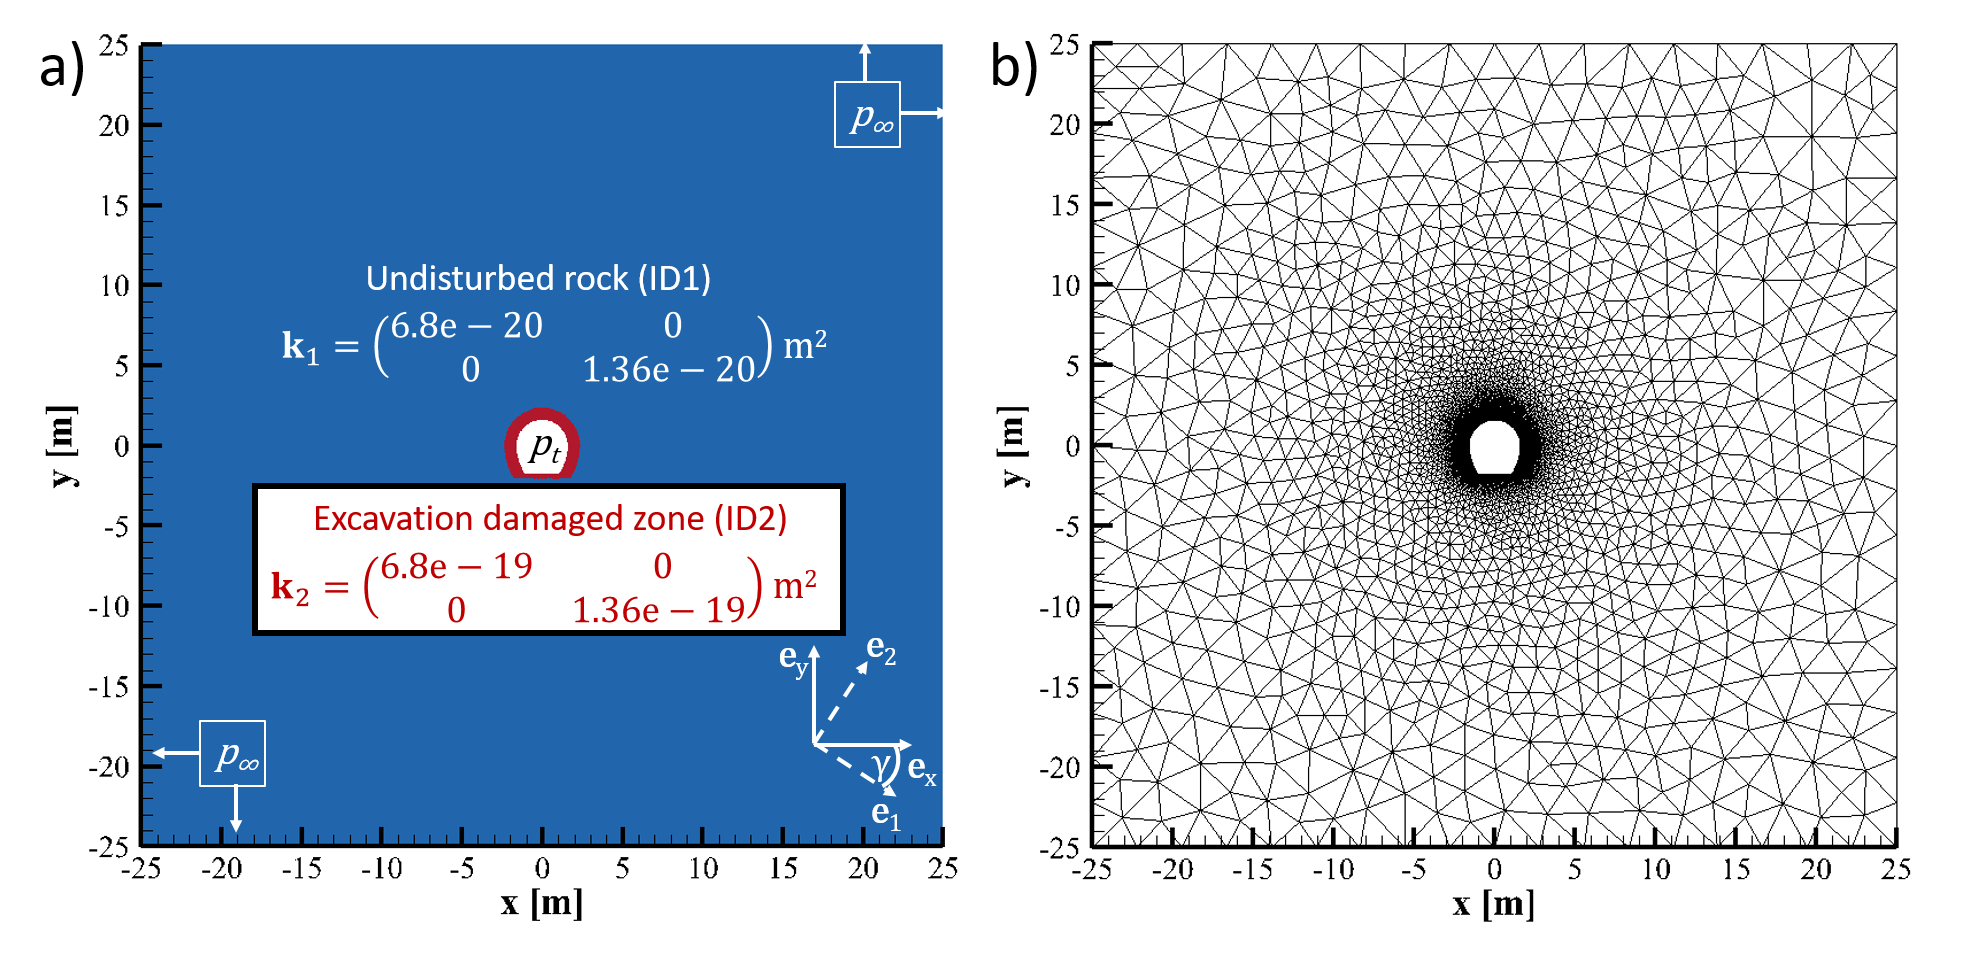
\includegraphics[width=\textwidth, trim=0.4cm 0 0 0, clip]{./figures/MEX10_setup_and_grid.png}
\caption{a) Computational setup and material parameters of the physical problem. b) Triangulated computational grid comprising 5463 nodes. }
\label{fig:setup}
\end{figure}

\begin{figure}
\centering
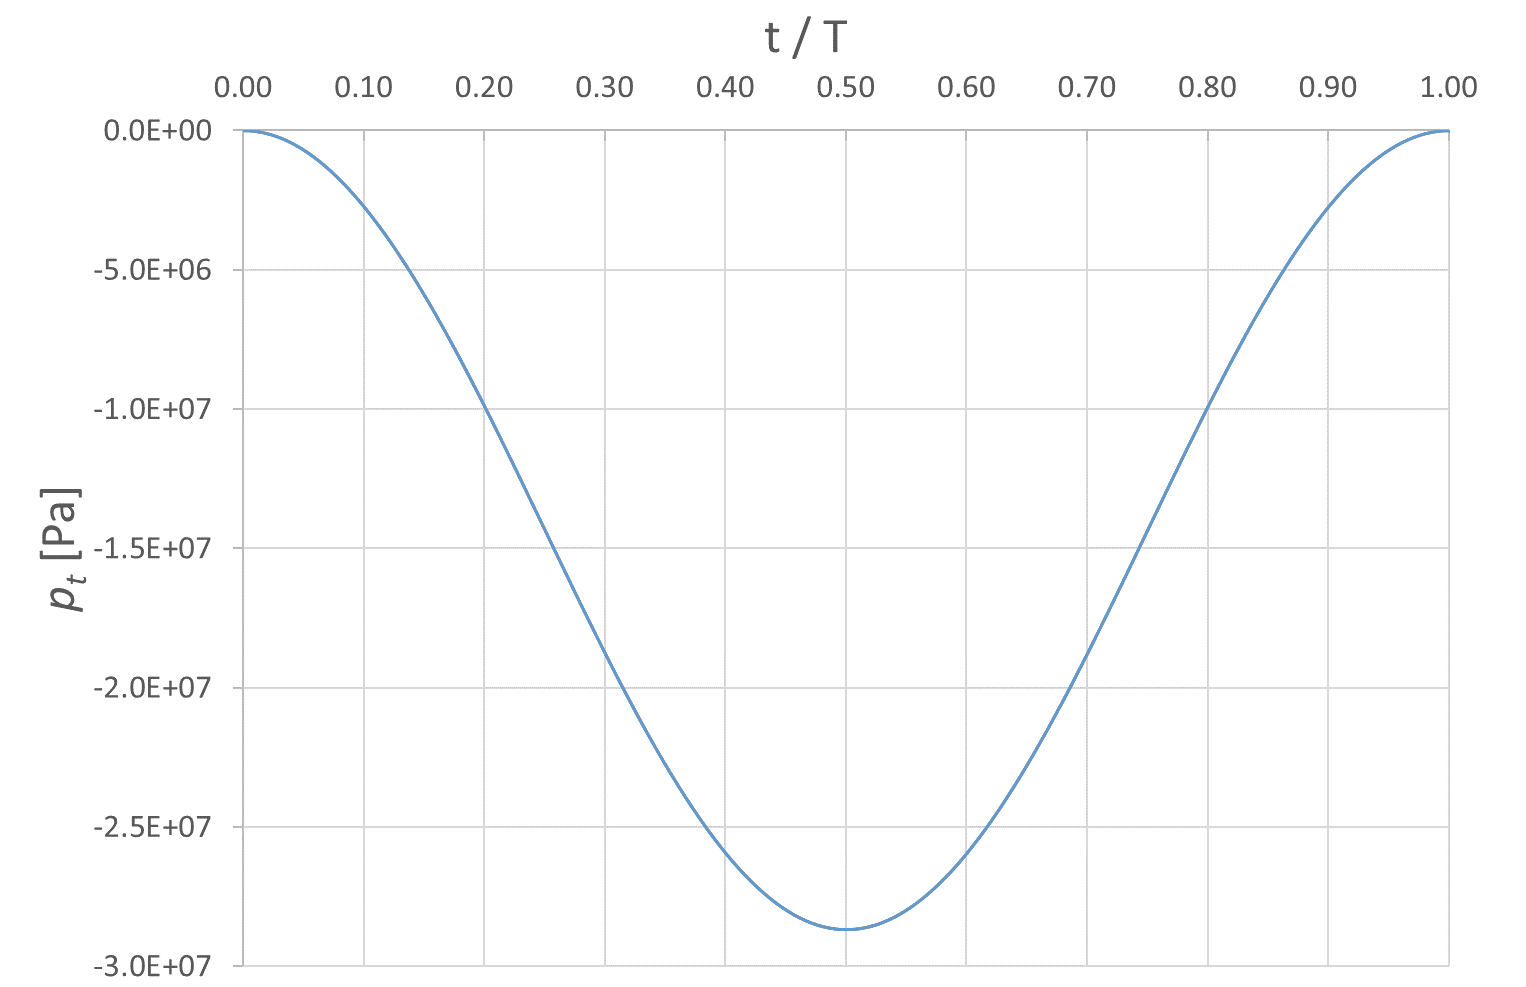
\includegraphics[width=0.7\textwidth]{./figures/MEX10_boundary_condition_tunnel.png}
\caption{Temporal evolution of the dynamic boundary condition at the wall of the niche for one seasonal period $T$. The total simulation time was ${T_\text{tot}=20T}$.}
\label{fig:bc}
\end{figure}

The simulation is set up as a two-dimensional problem. The total extent of the domain is 50 by 50 meters and the domain is discretized by a total of 5463 nodes with elements of triangular shape (Figure \ref{fig:bc}b) unless specified otherwise. This spatial discretization is the exact same mesh as used by \cite{ziefle2018}. A summary of the boundary conditions for the computational domain and the material parameters is given in Figure \ref{fig:setup}a. The seasonal change in pressure boundary conditions at the surface of the niche is shown as a function of time in Figure \ref{fig:bc}. The numerical parameters for the nonlinear and linear solver are listed in Table \ref{tab:solver}.


\begin{table}
 \caption{Numerical parameters of the solvers used in OGS-5 and OGS-6, where $\bf{r}$ and $\bf{b}$ are the residual and the right-hand side vector, respectively, and $\epsilon$ the error tolerance. Further the abbreviations for the solvers and preconditioners mean Conjugate Gradient on the Normal Equations (CGNR), Biconjugate gradient Stabilized Method (BiCGSTAB), and Incomplete LU Factorization Technique (ILUT), respectively.\label{tab:solver}}
\begin{center}
\begin{tabular}{ l | c | c || l | c | c }
 \multicolumn{3}{c||}{Nonlinear solver}			 & 	 \multicolumn{3}{ c}{Linear solver} \\
 Parameter 					& OGS-5 		& OGS-6	 & Parameter 			& OGS-5 			& OGS-6	\\
 \hline
 Solver  	 			& Picard 	& Picard & Solver  	 	& CGNR 		& BiCGSTAB \\ 
 Error 						& L2-norm 		& L2-norm  & Error 			& $\Vert\bf{r}\Vert<\epsilon \Vert\bf{b}\Vert$  	& $\Vert\bf{r}\Vert<\epsilon \Vert\bf{b}\Vert$  	\\		
  Error tol. $\epsilon$  	& 1E-5		& 1E-12  & Precon.	& Jacobi		& ILUT\\ 
  Max. iter.			& 50		& 40 	 & Error tol. $\epsilon$		& 1E-12			& 1E-10\\ 
 Relaxation					& 0.0		& n/a	 & Max. iter.	& 20000			& 3000 
\end{tabular}
\end{center}
\end{table}

%%%%%%%%%%%%%%%%%%%%%%%%%%%%%%%%%%%%%%%%%%%%%%%%%%%%%%%%%%%%%%%%%%%%%%%%%%%%%%%%%%%%%%%%%
\subsubsection{Well-developed stage}\label{sec:well_developed}
%%%%%%%%%%%%%%%%%%%%%%%%%%%%%%%%%%%%%%%%%%%%%%%%%%%%%%%%%%%%%%%%%%%%%%%%%%%%%%%%%%%%%%%%%
This well-developed stage is reached after 15 cycles of alternating wet and dry boundary conditions, i.e. 15 years of simulation time. The spatial distribution of $p_f$ and $S_\text{eff}$ is illustrated in Figure \ref{fig:results} for the results generated by OGS-5. Figures \ref{fig:results}a and b show the spatial distribution of the fluid pressure at a dry and a wet phase, respectively. Owing to the variations in pressure $p_t$ at the niche, i.e. relative air humidity inside the gallery,  the rock undergoes cyclic saturation and desaturation. As expected, this affects the saturation at the walls of the niche and in the vicinity of the walls. Farther away  from the boundary, a stable pattern develops for $p_f$ and $S_\text{eff}$ that reflects the transverse isotropic permeabilities prescribed by \eqref{eq:permeabilities}.  Even though the effect of desiccation becomes obvious in concentric ellipses surrounding the niche, the temporal evolution of the boundary condition at the wall of the niche is visible within the EDZ only. At this well-developed stage, the rest of the domain remains unaffected from these changes in $p_t$. The same can be observed for the effective saturation in Figures \ref{fig:results}c and d. Due to the nonlinear dependency of $S_\text{eff}$ and $p_f$ in \eqref{eq:cap_p}, the area that is substantially influenced by the seasonal variation of $p_t$ is even smaller in figures \ref{fig:results}c and d compared to figures \ref{fig:results}a and b.
%
\begin{figure}[t]
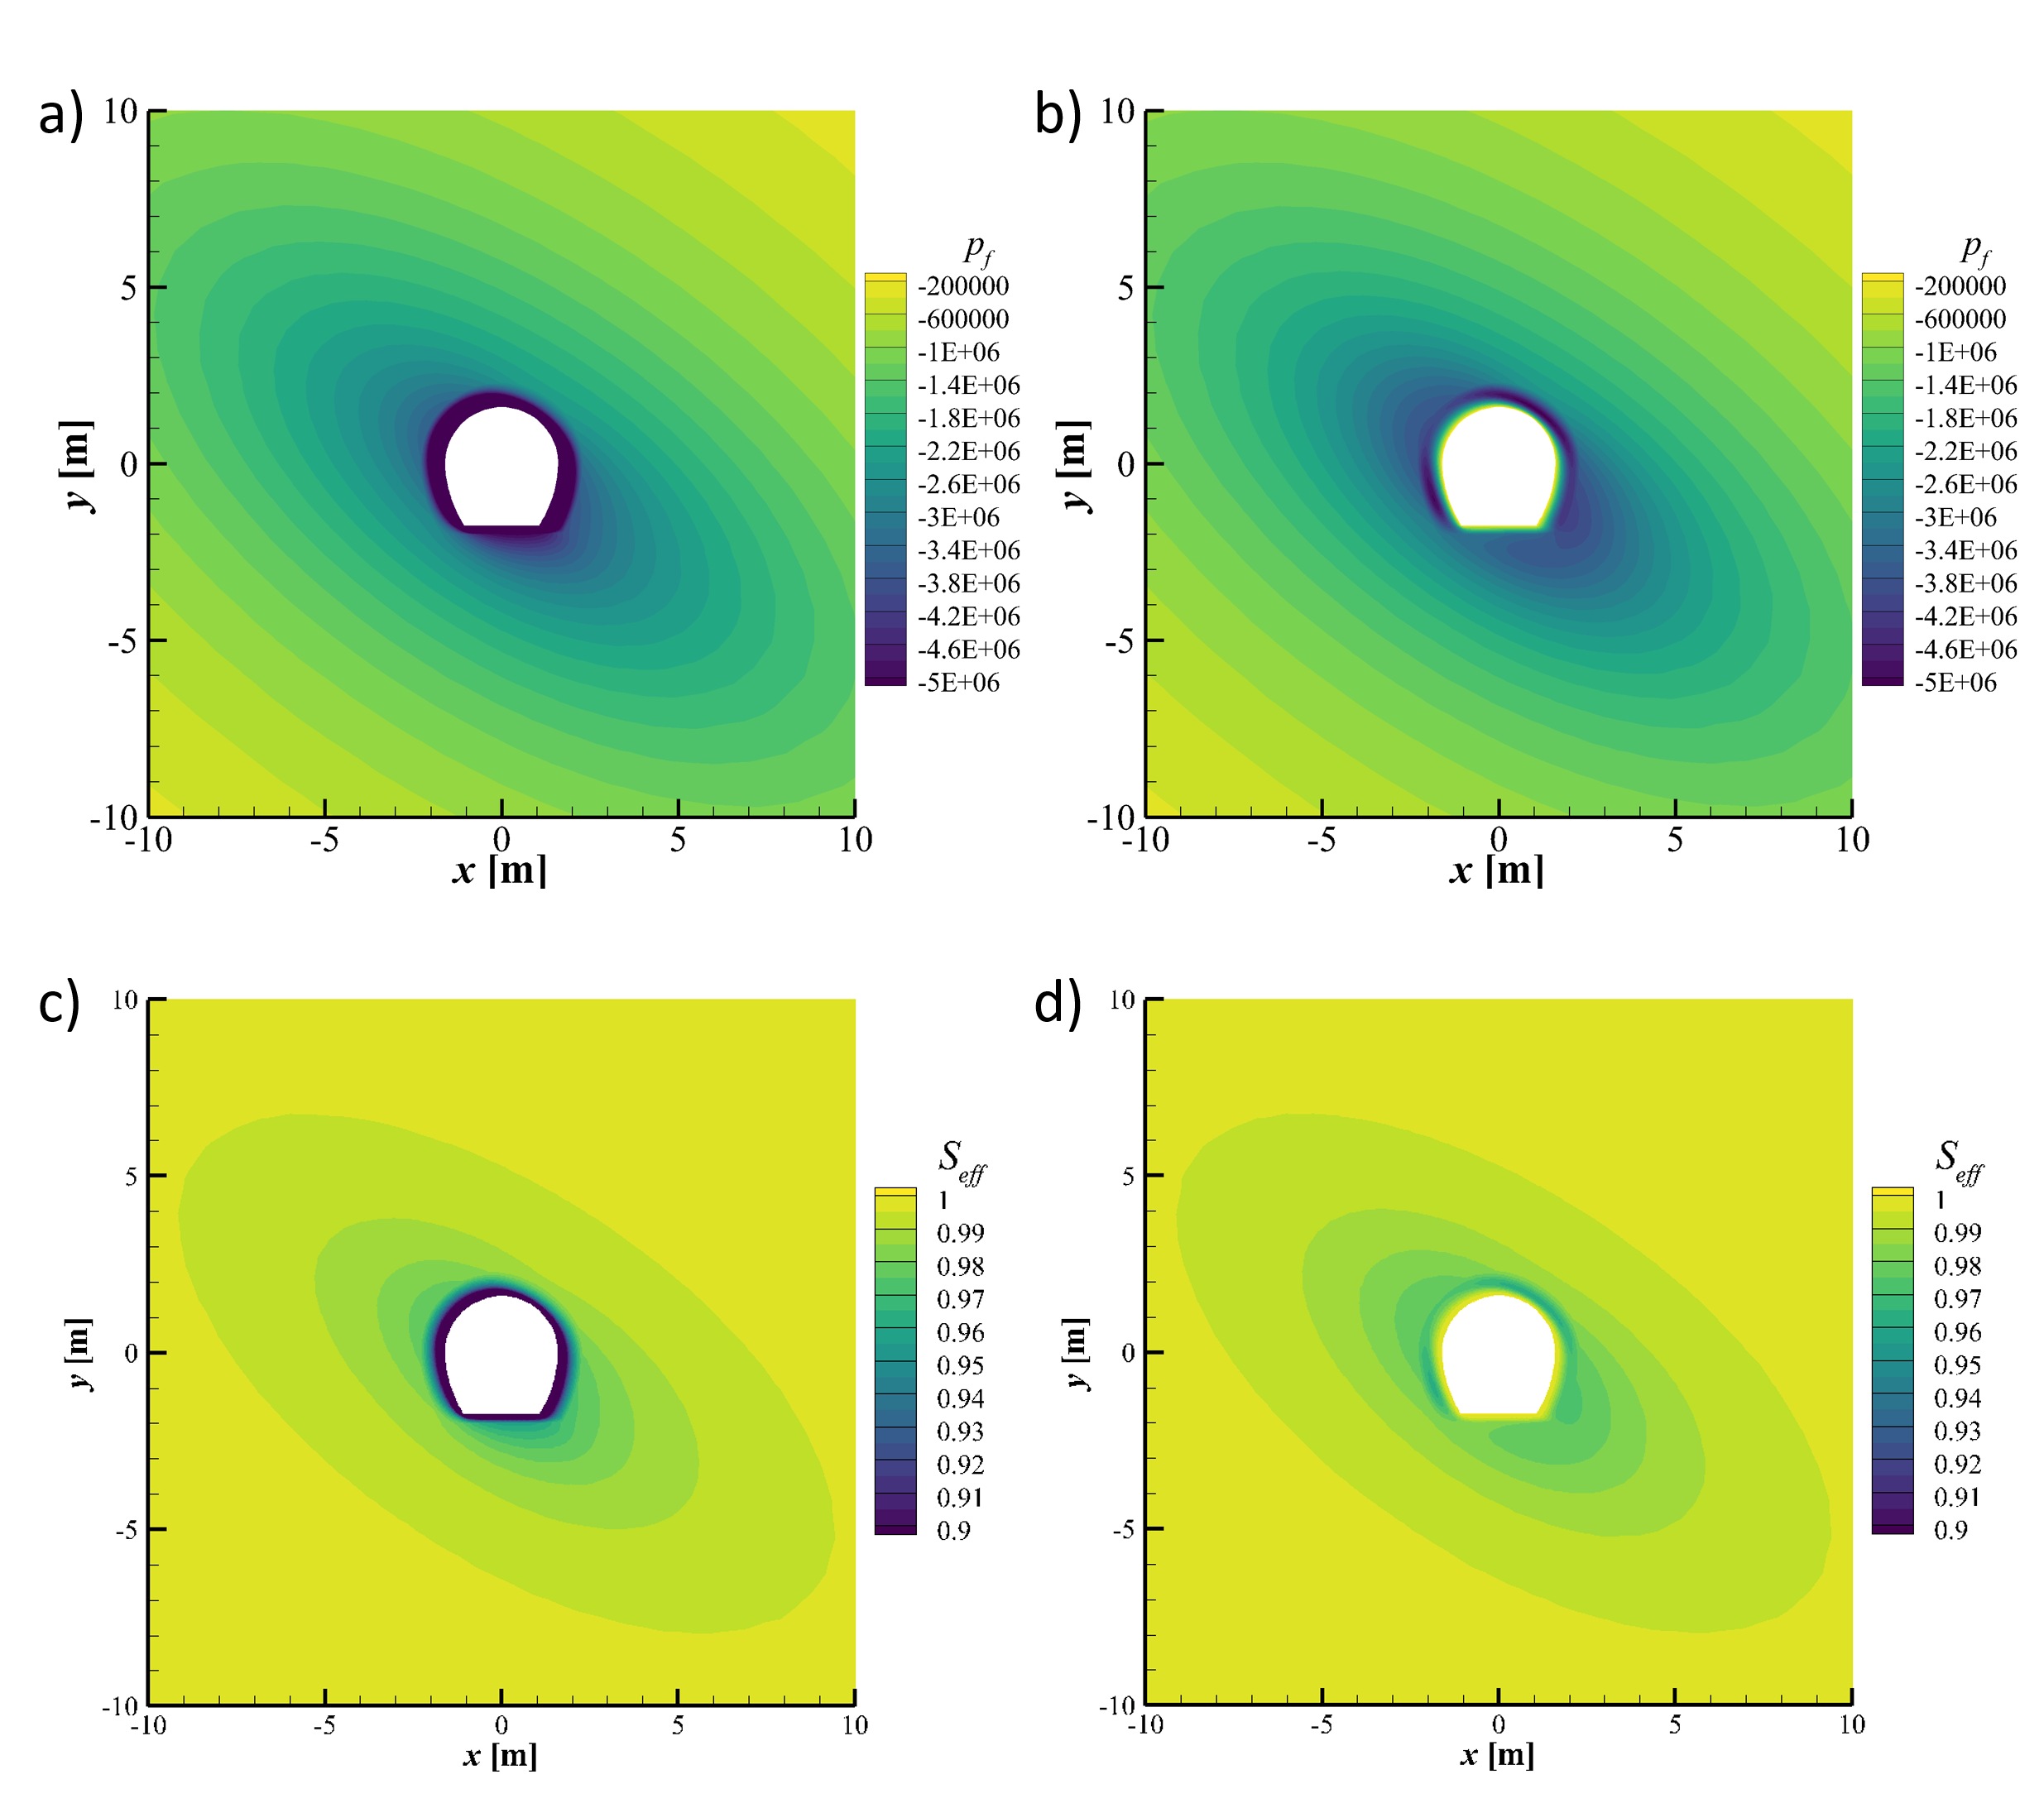
\includegraphics[width=\textwidth, trim=0.4cm 0.2cm 0.2cm 0, clip]{./figures/MEX10_results_pf_S.png}
\caption{Well-developed pattern of seasonally varying quantities fluid pressure (in Pa) and effective saturation. a) fluid pressure at $t=19.5\text{a}$, and b) fluid pressure at $t=20\text{a}$, c) effective saturation at $t = 19.5\text{a}$ and d) effective saturation at $t=20\text{a}$. The figures show a zoom into figure \ref{fig:bc}.}
\label{fig:results}
\end{figure}
%

%%%%%%%%%%%%%%%%%%%%%%%%%%%%%%%%%%%%%%%%%%%%%%%%%%%%%%%%%%%%%%%%%%%%%%%%%%%%%%%%%%%%%%%%%
\subsubsection{Comparison of OGS-5 and OGS-6}\label{sec:mex10_ogs5_vs_ogs6}
%%%%%%%%%%%%%%%%%%%%%%%%%%%%%%%%%%%%%%%%%%%%%%%%%%%%%%%%%%%%%%%%%%%%%%%%%%%%%%%%%%%%%%%%%

A more detailed insight into the evolution of the the desaturated rock surrounding the niche is revealed by plotting $p_f$ and $S_\text{eff}$ probed over time at four different points around the niche. This analysis is shown in Figure \ref{fig:cf_P_S} together with the locations of the sampling points as an inset. The seasonal variations are clearly visible, and the plot reaches a quasi-steady state after 15 years of simulation time. Hence, we conclude that the simulation ran long enough to reach a quasi-steady state for the zone surrounding the niche. Note, however, that these data were collected at locations 3 m away from the niche center in both, horizontal and vertical direction. For probing locations farther away from the niche, it takes longer  to reach a steady state. This state, however, will be closer to fully saturated conditions the farther one moves away from the niche into the undisturbed rock. 

It is now interesting to compare the results from both simulation codes, OGS-5 and OGS-6, to verify whether or not the results have changed after the new implementation of \eqref{eq:richards} in OGS-6. Hence, we show a direct comparison of the simulation results generated by OGS-5 and OGS-6 in the same figure (Figure \ref{fig:cf_P_S}). As desired, all data curves collapse for OGS-5 and OGS-6 at the four different locations for the time simulated. 

%
\begin{figure}[t]
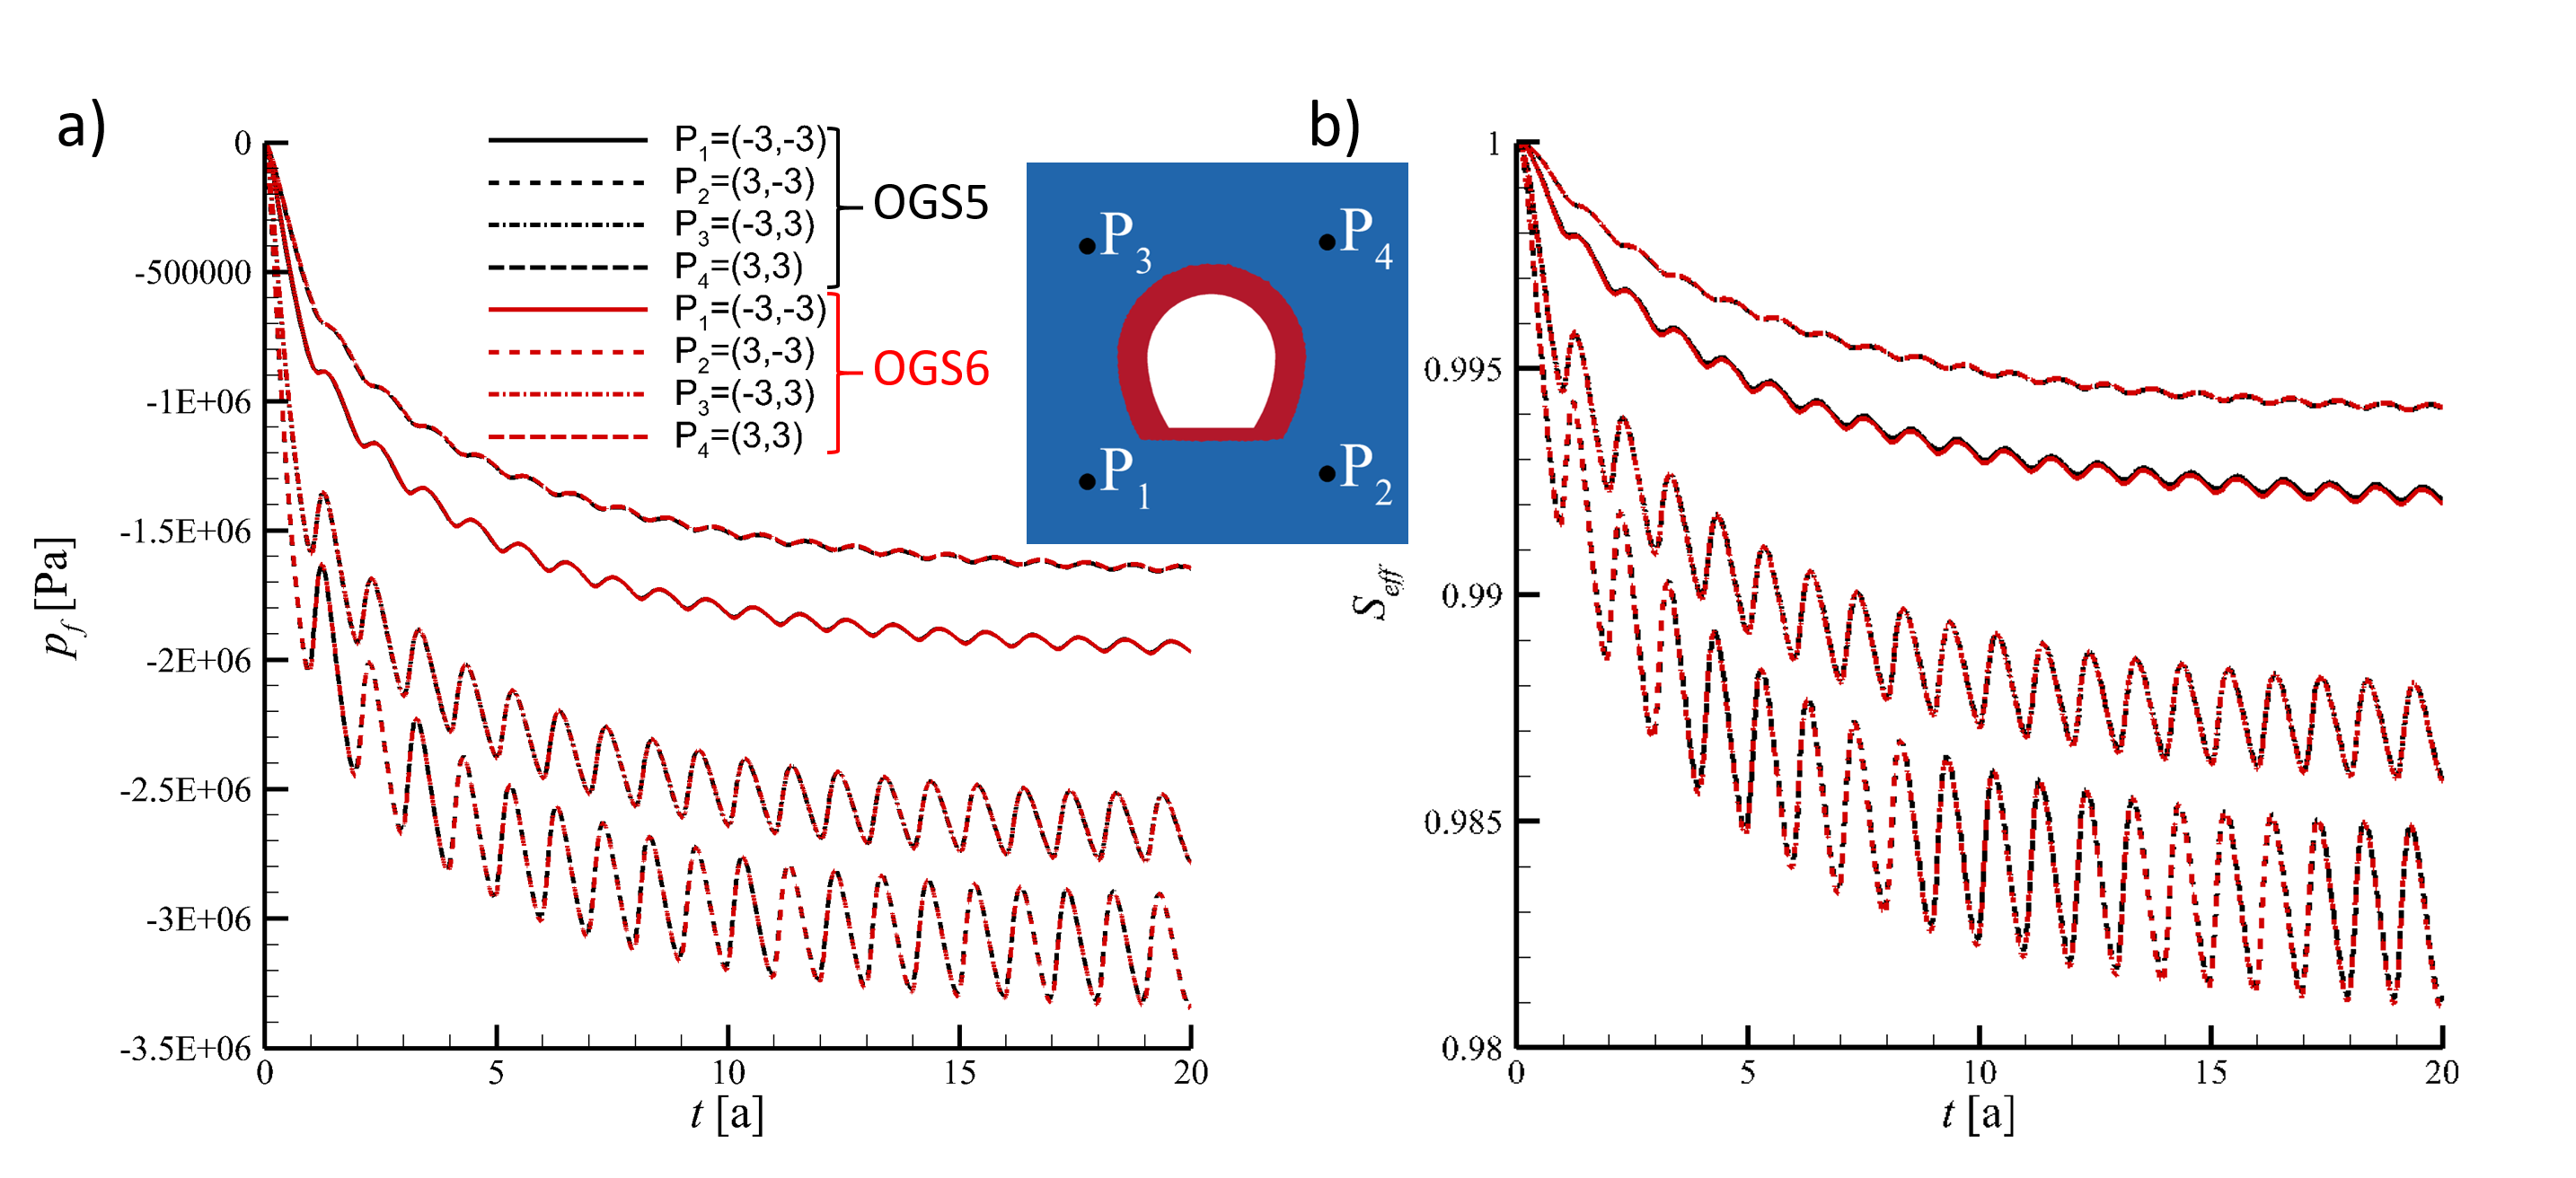
\includegraphics[width=\textwidth, trim=0.4cm 0.2cm 0.2cm 0, clip]{./figures/MEX10_cf_P_S.png}
\caption{Physical quantities probed over time at four different locations surrounding the niche for OGS-5 (black) and OGS-6 (red): a) Fluid pressure and b) effective saturation.  The inset shows the location of the sampling points relative to the niche. The results collapse for OGS-5 and OGS-6.}
\label{fig:cf_P_S}
\end{figure}
%

For a more quantitative comparison, we compute the relative deviation
%
\begin{equation}\label{eq:error}
\epsilon_\theta = \frac{\theta^{OGS5}-\theta^{OGS6}}{\theta^{OGS5}}
\end{equation}
%
where $\theta$ is a quantity of interest, e.g. $p_f$ or $S_\text{eff}$. The two-dimensional plot of the error is shown in Figure \ref{fig:error} for both of these quantities at time $t=20\text{a}$. Far away from the wall of the niche, the error remains small (below $0.1\%$). However, we obtain that OGS-6 slightly underestimates the pressure in the EDZ compared to OGS-5 (Figure \ref{fig:error}a). This is most pronounced at the edges that are not pointing in the main direction of the anisotropy, i.e. at the top right and bottom left edges of the wall. Similarly, we see deviations for the saturation, but here, $S_\text{eff}$ is underestimated at the wall and at the transition from the EDZ to the undisturbed rock, whereas it is overestimated in OGS-6 compared to OGS-5 within the rest of the EDZ (Figure \ref{fig:error}b).

\begin{figure}[t]
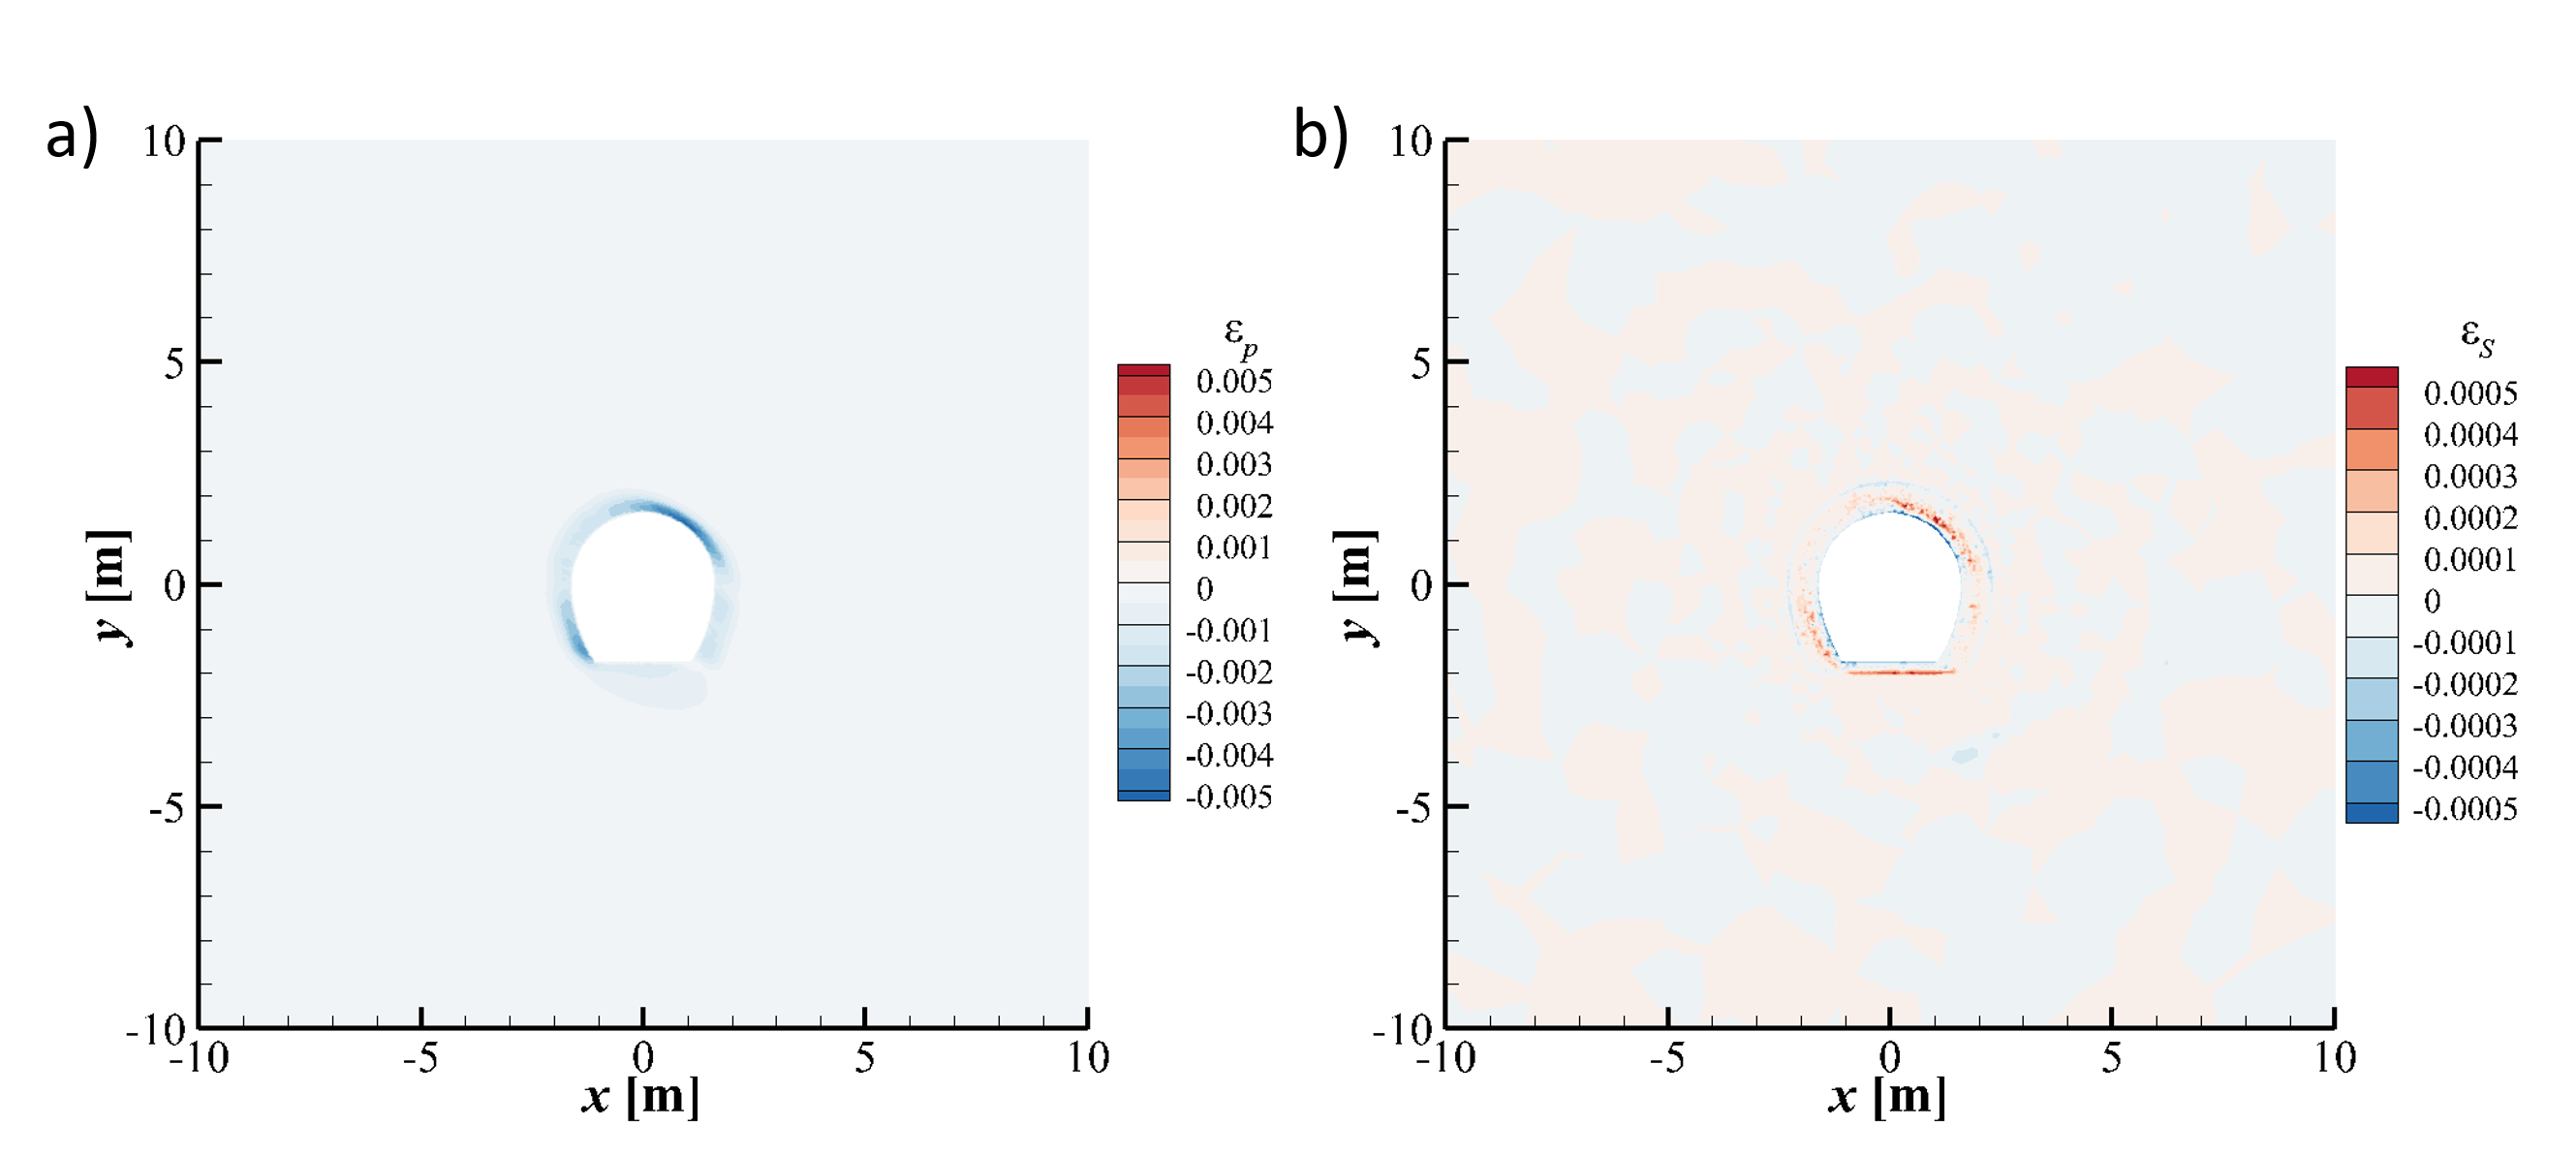
\includegraphics[width=\textwidth, trim=0.6cm 0.0cm 0.0cm 0.2cm, clip]{./figures/MEX10_cf_P_S_2D.png}
\caption{Deviation between OGS-5 and OGS-6 after 20 years of simulation time. a) Fluid pressure and b) effective saturation.}
\label{fig:error}
\end{figure}

Nevertheless, the maximum and minimum deviations as well as the RMSE
\begin{equation}\label{eq:RMSE}
\left \langle \left \lvert \overline{\epsilon}_\theta \right \rvert \right \rangle = \text{RMSE}=\frac{1}{N_\text{nodes}}\sum_{i=1}^{N_\text{nodes}} \sqrt{\epsilon_\theta^2}
\end{equation}
remain below $0.1\%$  (Table \ref{tab:error}). Here, RMSE is the Root Mean Square Error, $i$ is the index of the nodes, and $N_\text{nodes}$ is the total number of nodes of the computational mesh. These small deviations were deemed to be acceptable for the present scenario given that the simulation had run more than twenty cycles of desiccation/saturation.  This is especially true considering the different convergence criteria used for the two different codes (Table \ref{tab:solver}). 

\begin{table}
 \caption{Deviations observed when comparing OGS-5 with OGS-6 for the RF model.\label{tab:error}}
\begin{center}
\begin{tabular}{ l | c | c | c }
 Quantity			& $\min{(\epsilon)}$ 	& $\max{(\epsilon)}$	 & RMSE  \\
 \hline
 $p_f$ & -0.0054 	& 0.0 		& $5.52\cdot 10^{-5}$\\ 
 $S_\text{eff}$ & -0.0012 & 0.0078	& $6.77\cdot 10^{-4}$\\		
\end{tabular}
\end{center}
\end{table}

%%%%%%%%%%%%%%%%%%%%%%%%%%%%%%%%%%%%%%%%%%%%%%%%%%%%%%%%%%%%%%%%%%%%%%%%%%%%%%%%%%%%%%%%%
\subsubsection{Convergence study in space and time in OGS-6}
%%%%%%%%%%%%%%%%%%%%%%%%%%%%%%%%%%%%%%%%%%%%%%%%%%%%%%%%%%%%%%%%%%%%%%%%%%%%%%%%%%%%%%%%%
The rate of convergence is a very important property to jugde the consistency of a numerical procedure. A consistent procedure approaches the analytical solution of the problem with increasing resolution in space and time \cite{ferziger2012}.  For an efficient numerical scheme, the rate of convergence should be equal to or greater than unity, i.e. dividing the resolution by a factor of two should also decrease the error by at least a factor of two with respect to the reference solution. By comparing the numerical solution to some reference solution, one can also infer information about the minimum resolution required to obtain acceptable results. While the rate of convergence is often times determined under ideal conditions, i.e. on a regular Cartesian grid for an idealized problem, we apply the procedure to the present case of a niche surrounded by rock of two material groups, anisotropic permeability and cyclic boundary conditions for the fluid pressure at the walls of the niche to analyze a more realistic scenario. This is done in two consecutive steps: first we present order of convergence in time and then in space. 

\subsubsection*{Convergence study time}
To analyze the consistency in time, we use the exact same computational setup described in Section \ref{sec:model_RF} above. While the results generated with this setup and presented in Sections \ref{sec:well_developed} and \ref{sec:mex10_ogs5_vs_ogs6} were computed with $\Delta t = 21,400$ s, we now vary the time integration interval within the range $1350 \, \text{s} \leq \Delta t  \leq 345,600$ s. We ran a total of nine simulations doubling $\Delta t$ for each simulation. This yields an integration time interval ranging between 24 minutes and 4 days. The run with the smallest time integration interval, i.e. $\Delta t = 1350$ s, was chosen as a reference solution, since there is no analytical solution available for the current setup.

\begin{figure}[t]
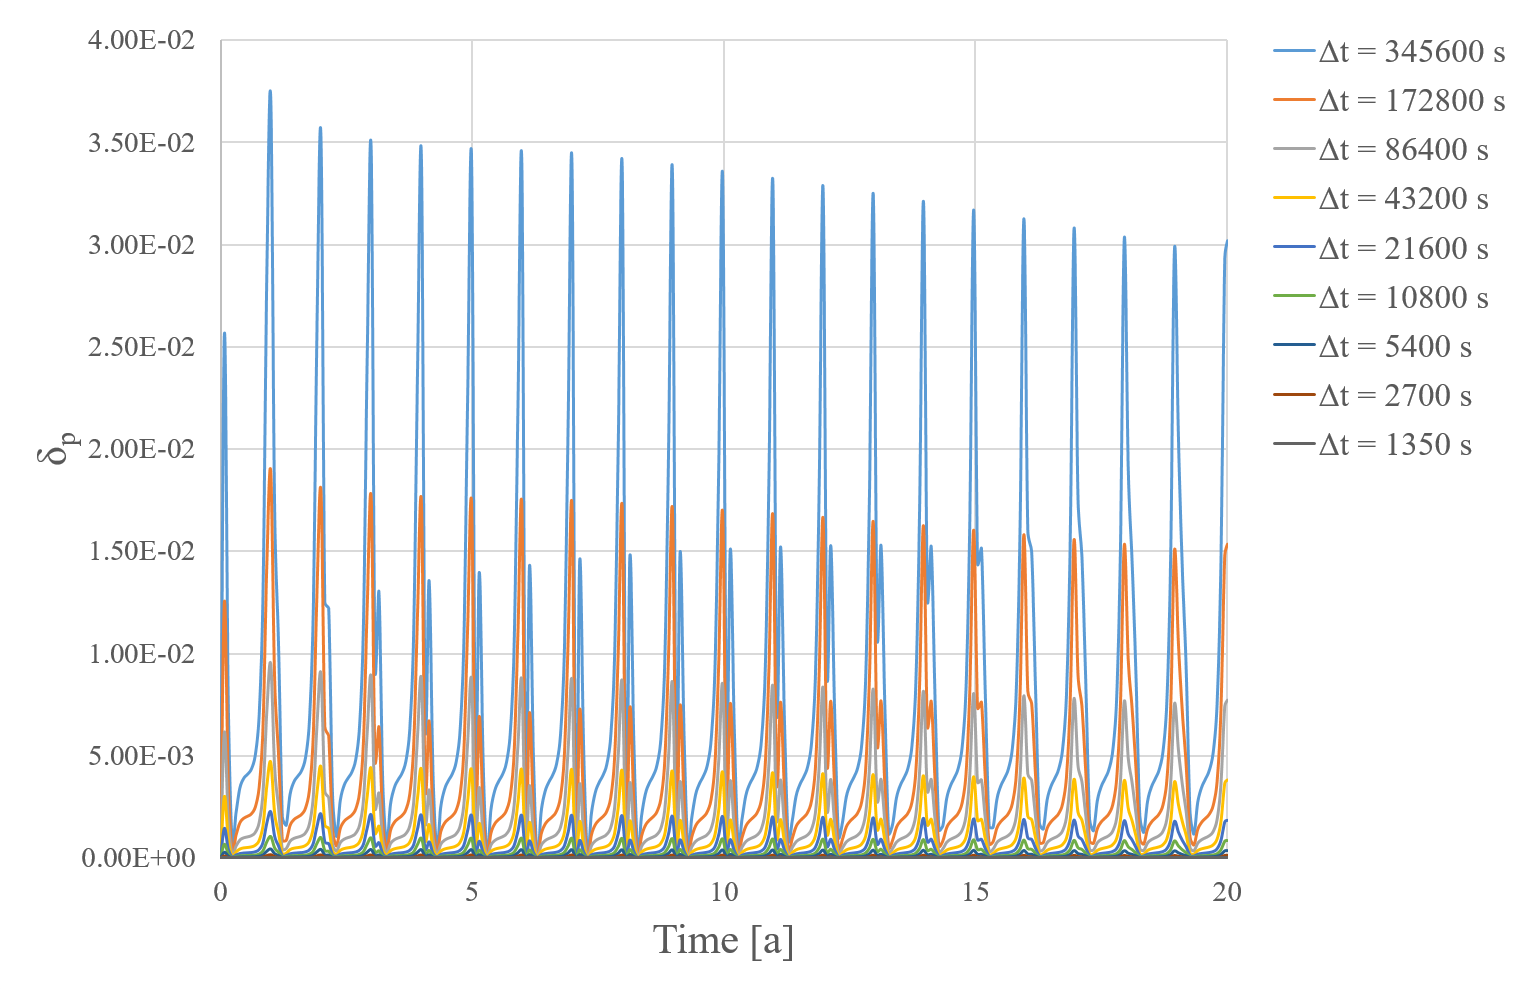
\includegraphics[width=\textwidth]{./figures/MEX10_convergence_error.png}
\caption{Deviation between the simulations using different time discretizations $\Delta t$ at sampling point $P_1 = (2.0,0.0)$ (cf. inset in Figure \ref{fig:convergence_time}). }
\label{fig:convergence_error}
\end{figure}

As a next step, we define sampling points, for which we probe data for fluid pressure and effective saturation over time.  Since Figure \ref{fig:error} suggested that deviations between OGS-5 and OGS-6 were largest at the transition zone from the undisturbed rock (material ID 1) to the EDZ (material ID 2), we chose four different locations inside the EDZ surrounding the niche at this critical distance, which is 2 m away from the domain center for $P_1, P_2$ and $P_3$ and 1.9 m for $P_4$, which is directly located underneath the niche. The  coordinates are sketched in the inset in Figure \ref{fig:convergence_time} and listed in Table \ref{tab:convergence_time}. As a next step, we define the characteristic error
%
\begin{equation}
\delta_\theta(\Delta t) = \left \lvert \frac{\theta(\Delta t) - \theta(\Delta t_\text{ref}) }{\theta(\Delta t_\text{ref})} \right \rvert \qquad ,
\end{equation}
%
where again $\theta$ represents fluid pressure and effective saturation, respectively, and $\Delta t_\text{ref}= 1350$ s is the time integration interval of the reference run. 

An example of the temporal evolution of $\delta_p$ for $P_1 = (2.0,0.0)$ is given in Figure \ref{fig:convergence_error}. Similar to the observations reported for Figure \ref{fig:bc} above, there is a strong cyclic behavior of the error that depends on the evolution of $p_t$. A peak in $p_t$ corresponds with a maximum deviation of the simulation result from the reference solution. This behavior was expected as a coarser discretization tends to smoothen out maximum values of a continuous function.  For a given $\Delta t$, the deviations slightly decrease over time and decreasing $\Delta t$ reduces the deviations from the reference solution substantially for all values of $\Delta t$ investigated. Similar results were obtained for the other three sampling points.

\begin{figure}[t]
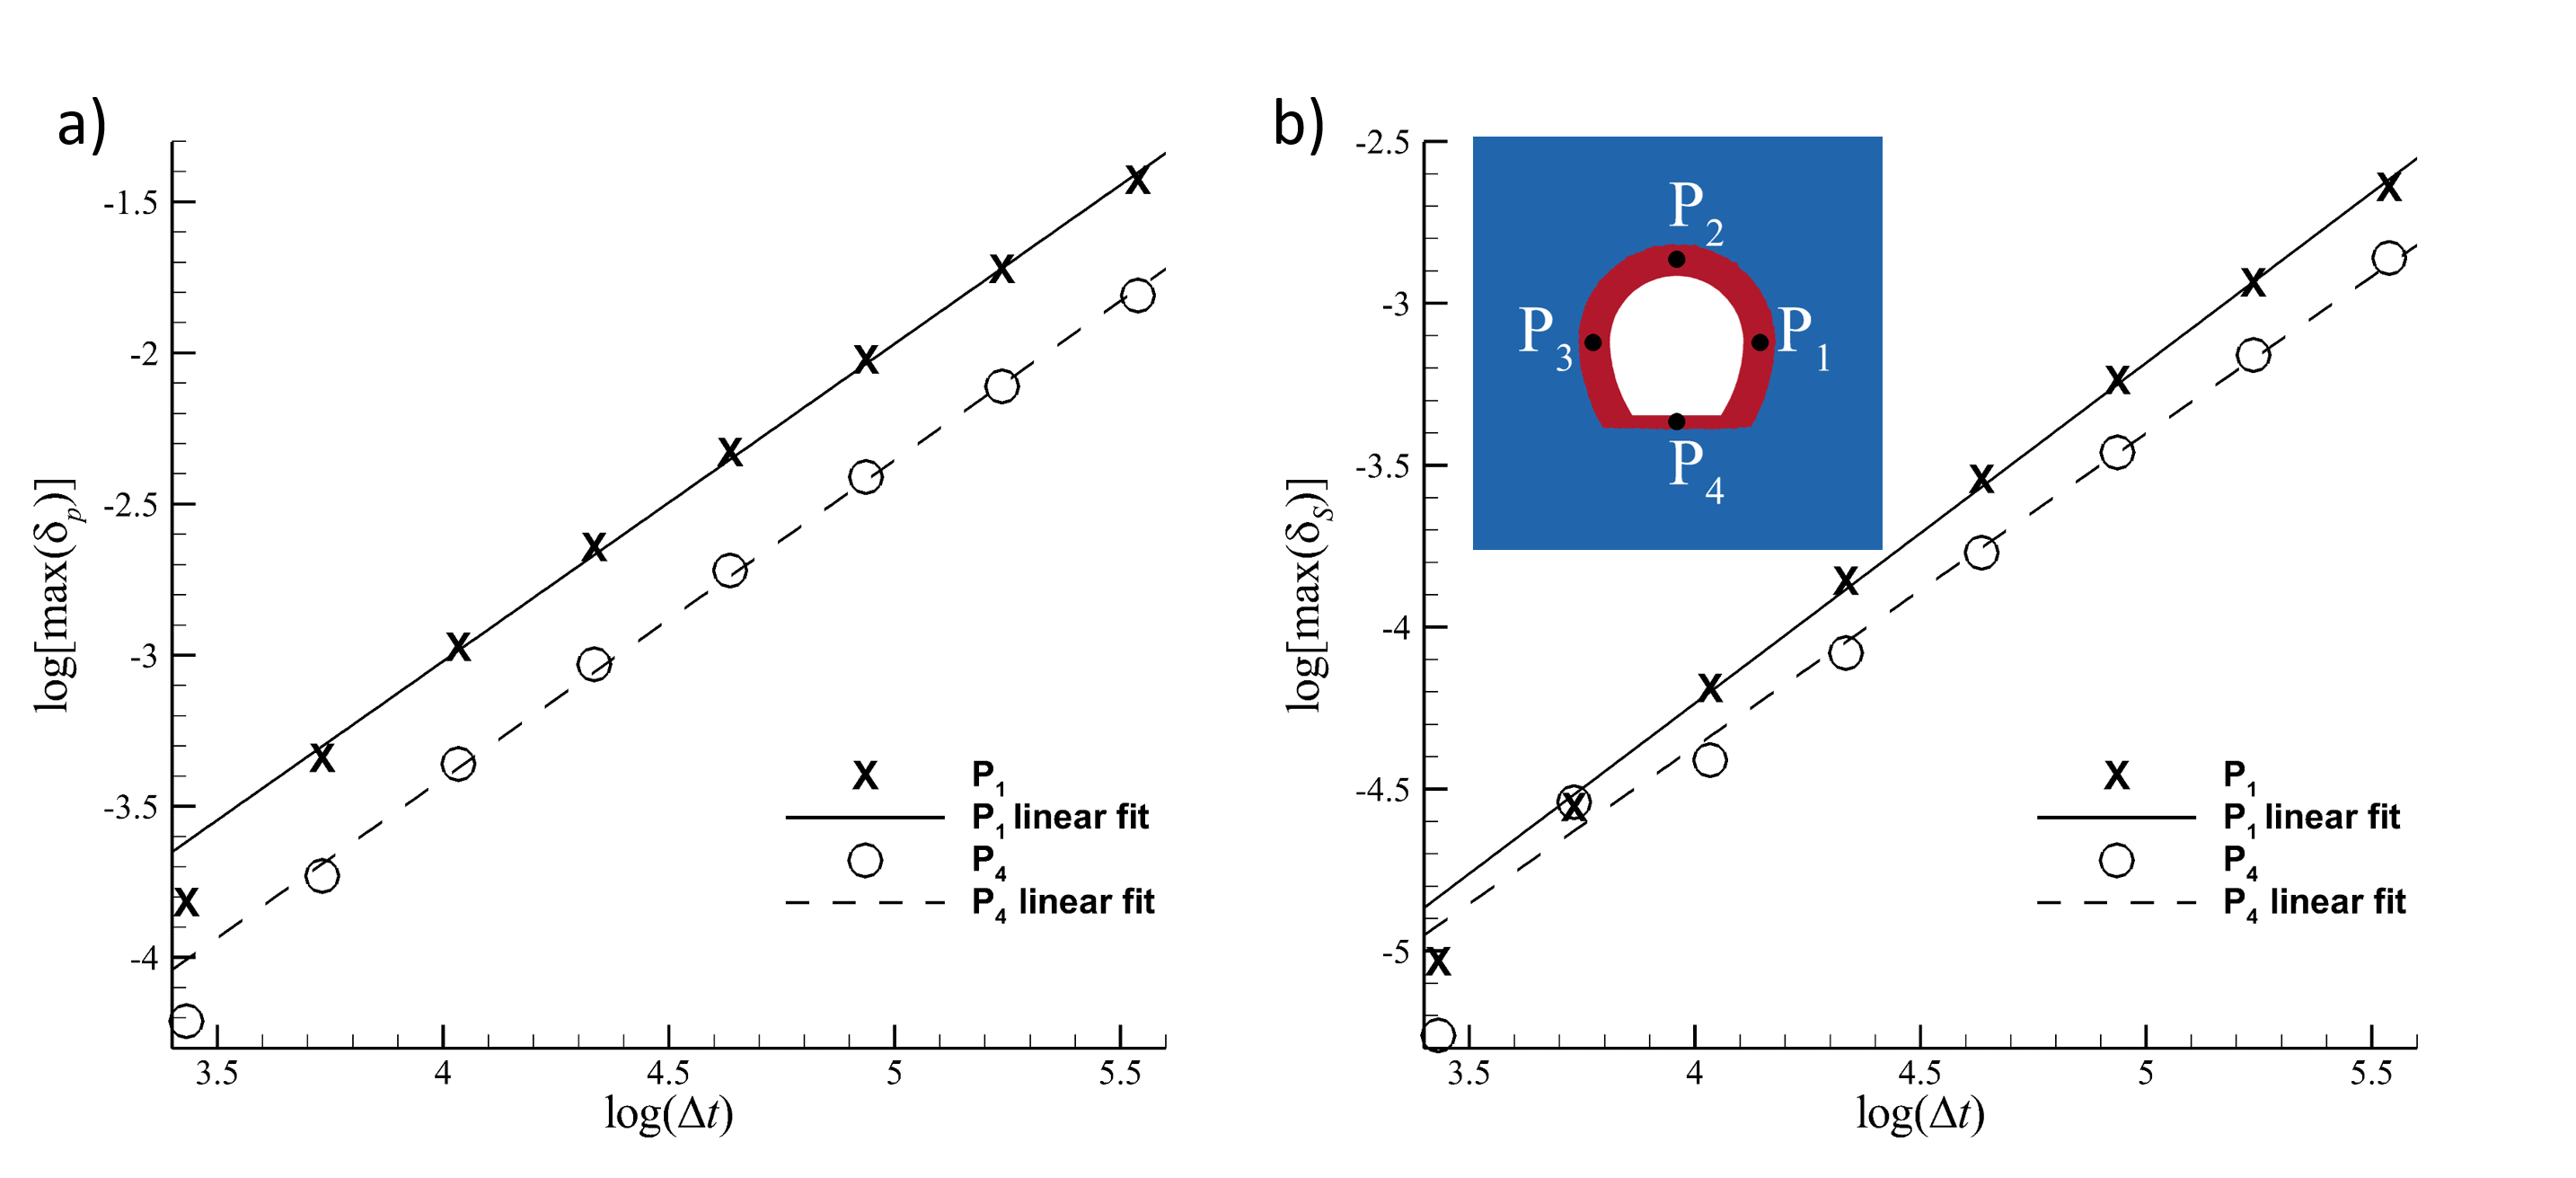
\includegraphics[width=\textwidth]{./figures/MEX10_convergence_time.png}
\caption{Order of convergence in time for two characteristic sampling points on a log-log scale. The error increases with increasing $\Delta t$. a) Fluid pressure and b) effective saturation. The inset shows the locations of the analyzed sampling points. }
\label{fig:convergence_time}
\end{figure}

To quantify the deviations from the reference solution, we plot the maximum deviation $\max{(\delta_\theta)}$ against $\Delta t$ in a log-log plot in Figure \ref{fig:convergence_time}. As already observed in Figure \ref{fig:convergence_error}, all data points follow the same trend of decreasing error with decreasing time step size. Note that we have only plotted results for $P_1$ and $P_4$, because the data from $P_2$ and $P_3$ collapsed with the data from $P_1$. The offset of $P_4$ from the rest of the sampling points is probably due to the slight difference in distance from the center of the domain and the flat bottom wall of the niche.


Finally, we determine the order of convergence by computing the linear fit of $y=ax + b$ for the log-log plot in Figure \ref{fig:convergence_time}. In fact, the linear fit is a very good approximation of the data presented in that figure, so that the fitting parameter $a$, which is the slope of the linear regression, serves very well to determine the order of convergence. Note that we have excluded the first data point (with the lowest value of $\Delta t$) from the fit, because it is slightly offset due to the fact that the reference case using $\Delta t_\text{ref}$ does not represent an analytical solution as would have been desirable for a mathematically rigorous convergence analysis. The values of $a$ and $b$ for the fluid pressure and the effective saturation are summarized in Table \ref{tab:convergence_time} for all four sampling points investigated.  For both physical quantities, the slope turns out to be 1.05 on average, which proves that the current time integration scheme of the "Richards Flow" model in OGS-6 is an efficient implementation of the {\em Backward Euler} scheme; a scheme that is known to be of first order \cite{ferziger2012}. 

\begin{table}
 \caption{Order of convergence in time extracted from the linear fit $y=ax + b$ as given in the log-log plot of Figure \ref{fig:convergence_time} at the different sampling points shown in the same figure.\label{tab:convergence_time}}
 \begin{center}
\begin{tabular}{ l || r | r ||  r | r }
 					& \multicolumn{2}{c ||}{Pressure} & \multicolumn{2}{c}{Saturation} \\
Sampling point		& $a$ 		& $b$ 	    & $a$		& $b$ \\
 \hline
 $P_1=(2.0,0.0)$ 	& 1.051 	& -7.222 	& 1.052 	& -8.441 	\\ 
 $P_2=(0.0,2.0)$ 	& 1.050  	& -7.217	& 1.107 	& -8.715 	\\ 
 $P_3=(-2.0,0.0)$ 	& 1.046 	& -7.192	& 1.054 	& -8.431 	\\ 
 $P_4=(0.0,-1.9)$ 	& 1.054 	& -7.622	& 0.968 	& -8.242 	\\ 
\end{tabular}
\end{center}
\end{table}


\subsubsection*{Convergence study space}
Similar to the convergence study in time described above, we use the computational setup described in Section \ref{sec:model_RF} to repeat the simulations on different grids with different resolution. This time, the time integration interval was kept constant at $\Delta t = 21,400$ s, but the number of grid nodes $N_\text{nodes}$ was varied within the range $3613 \leq N_{nodes} \leq 60,845$. Note that we switched from a triangulated domain to a tetrahedral meshing due to its more regular behavior for grid refinements at the walls of the niche. We conducted a total of five simulations, where the simulation with $N_\text{nodes}=3614$ used the coarsest grid (Figure \ref{fig:meshes}a), $N_\text{nodes}= 6500$ is comparable to the triangulated grid with 5463 nodes as shown in Figure \ref{fig:setup}b, while we refined the grid to $N_\text{nodes}=11,045$ (Figure \ref{fig:meshes}b) and $N_\text{nodes}=31,582$, respectivly. Again, the finest resolution with $N_\text{nodes}=N_\text{ref}=60,845$ (Figure \ref{fig:meshes}c) serves as the reference run, since there is no analytical solution available. 

It is important to note that the the mesh generator Gmsh \cite{geuzaine2009} does not allow for the exact control over the number of nodes generated for the complex geometry in the present analysis. Hence, we adapt the number of grid cells by refining the spatial discretization at the outer boundary of the domain from 5 m ($N_\text{nodes} = 3613$) to 0.7 m ($N_\text{nodes} = 60,845$). This measure did not refine the grid at the walls of the niche in the same systematic manner, because the nodes have to coincide with the points defining the polygon course of the complex niche shape. In fact, we obtained the same spatial resolution $\Delta x = 0.0375$ m for the arch of the niche for all simulations, whereas the resolution at the more regular bottom was refined from 0.177 m to 0.034 m. 

\begin{figure}[t]
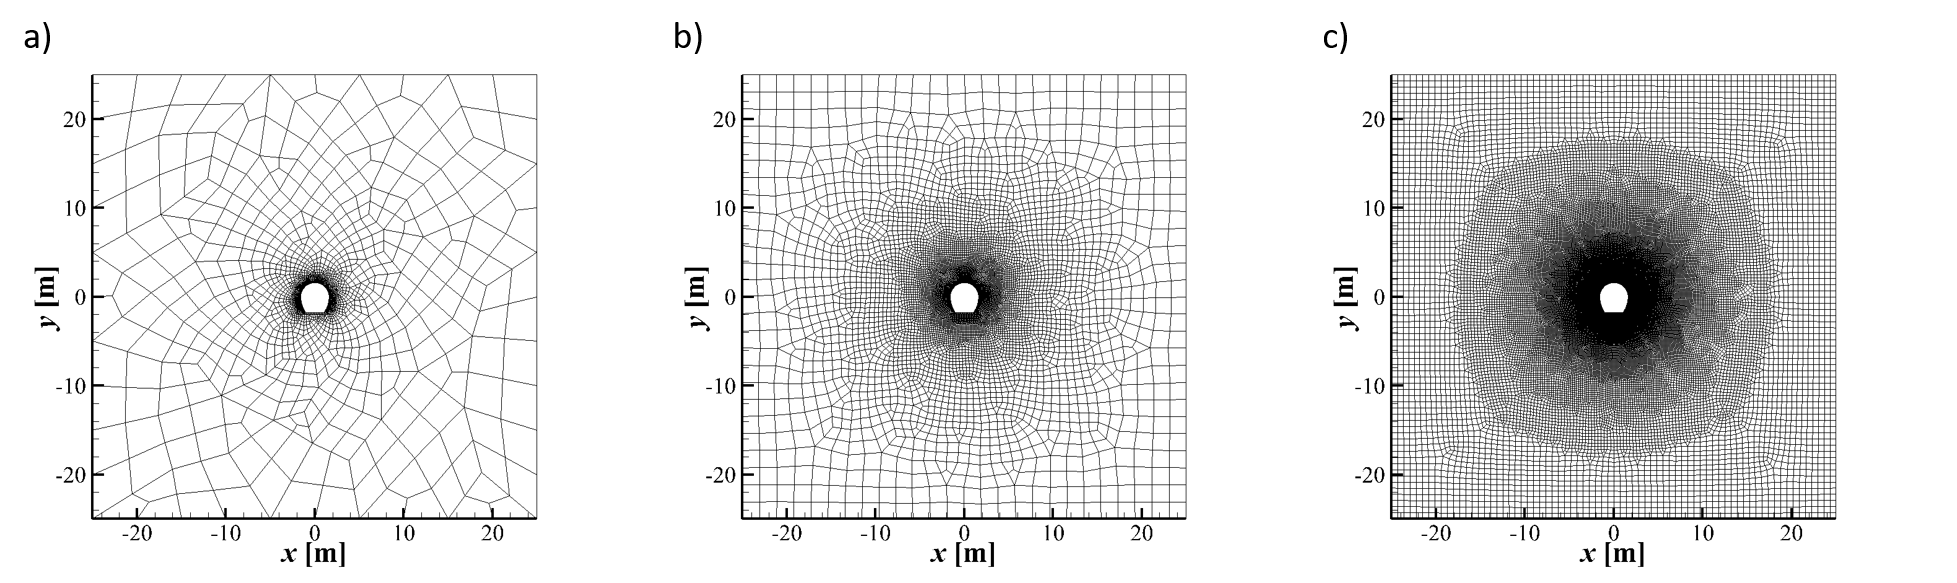
\includegraphics[width=\textwidth, trim=0.4cm  0.0cm 0 0.3cm, clip]{./figures/MEX10_meshes.png}
\caption{Examples of the meshes used to conduct the grid convergence. a) $N_\text{nodes}=3613$, which was the coarsest grid employed, b) $N_\text{nodes}=11,047$, c) $N_\text{nodes}=60,845$, which was the finest grid employed.}
\label{fig:meshes}
\end{figure}

We compute the error as 
%
\begin{equation}
\delta_\theta(N_\text{nodes}) = \left \lvert \frac{\theta(N_\text{nodes}) - \theta(N_\text{ref}) }{\theta(N_\text{ref})} \right \rvert \qquad ,
\end{equation}
%
to quantify the deviation of the results with respect to a given reference mesh, here the finest spatial resolution with $N_\text{ref}=60,845$ nodes. We defined four sampling points that were moved farther into the undisturbed rock to a distance of 4 m away from the center of the niche (Figure \ref{fig:convergence_space}). This became necessary as the polyline defining the boundary between the two material IDs, which is about 2 m away from the center of the niche, predefines specific nodes. Sampling in this area would influence the convergence behavior of the simulations. Subsequently, we used a interpolation routine provided by the software TecPlot \cite{tecplot2019} to obtain data over time at these sampling points for all the simulations with different grid resolution. Due to the remeshing, however, the sampling points' location no longer coincide with the node locations. Hence, if the grid is too coarse, those sampling points can be closer or farther away from the next node location depending on the mesh. For these cases, the interpolation routine offered by the postprocessing software TecPlot will heavily influence the results and conclusions about the order of convergence will no longer be possible.


\begin{figure}[t]
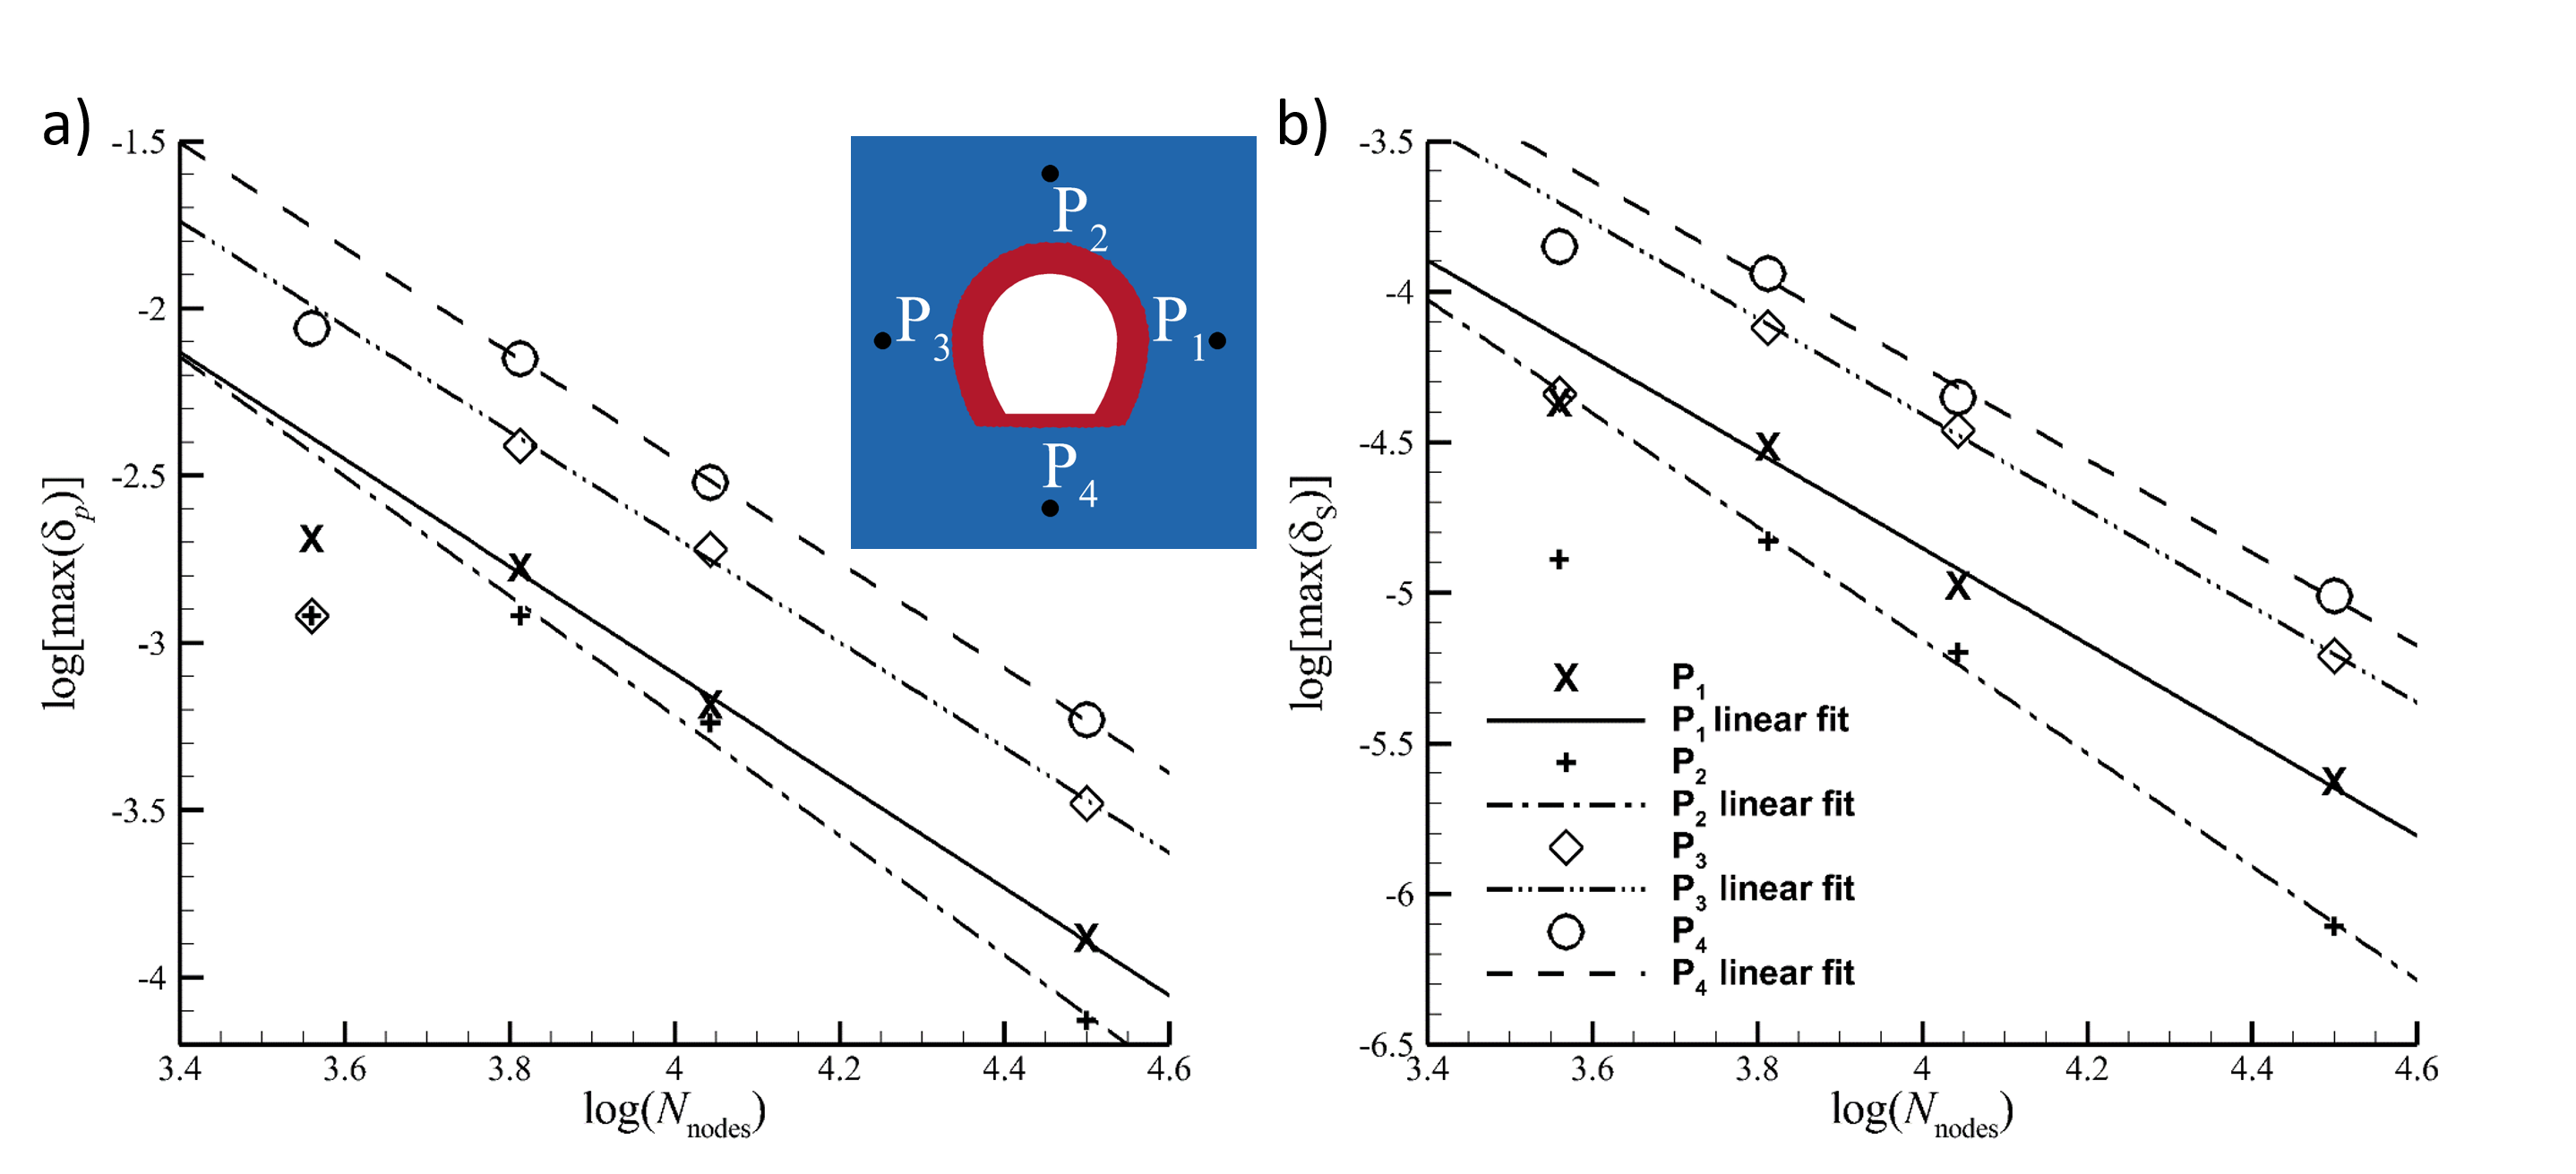
\includegraphics[width=\textwidth, trim=0.3cm  0.0cm 0 0.0cm, clip]{./figures/MEX10_convergence_space.png}
\caption{Order of convergence in space for four characteristic sampling points on a log-log scale. The error decreases with increasing number of grid cells $N_\text{nodes}$. a) Fluid pressure and b) effective saturation. The inset shows the locations of the analyzed sampling points. }
\label{fig:convergence_space}
\end{figure}

After probing the data at the different sampling points, we obtain results very similar to Figure \ref{fig:convergence_error}. The resulting convergence behavior with increasing grid resolution is shown in Figure \ref{fig:convergence_space} for both fluid pressure and effective saturation. Overall, the error decreases with increasing grid resolution. This is true for both quantities recorded at all four sampling points, except for the values recorded for the coarsest mesh with $N_\text{nodes}=3614$. Apparently, the interpolation routine of the postprocessing software has a big impact on the quality of the results of this run. It was therefore decided to exclude these data from the linear regression analysis and the grid with $N_\text{nodes} = 3613$ nodes was deemed to be too coarse to obtain meaningful results.

\begin{table}
 \caption{Order of convergence in space extracted from the linear fit $y=ax + b$ as given in the log-log plot of Figure \ref{fig:convergence_time} at the different sampling points shown in the same figure.\label{tab:convergence_space}}
 \begin{center}
\begin{tabular}{ l || r | r ||  r | r }
 					& \multicolumn{2}{c ||}{Pressure} & \multicolumn{2}{c}{Saturation} \\
Sampling point		& $a$		&$b$		& $a$		& $b$ \\
 \hline
 $P_1=(4.0,0.0)$ 	& -1.603 	& 3.321 	& -1.593  	& 1.521 	\\ 
 $P_2=(0.0,4.0)$ 	& -1.789 	& 3.938		& -1.883	& 2.374 	\\ 
 $P_3=(-4.0,0.0)$ 	& -1.574	& 3.611		& -1.596 	& 1.975 	\\ 
 $P_4=(0.0,-4.0)$ 	& -1.571 	& 3.836		& -1.543 	& 1.921 	\\ 
 
\end{tabular}
\end{center}
\end{table}

Nevertheless, after excluding two out of five simulations (with the coarsest being too coarse and the finest being the reference case), we are able to perform a linear regression analysis $y = ax + b$ with a very high correlation on the remaining three data points for the four different sampling locations. The slope of this linear regression, which is the fitting parameter $a$, then yields the order of convergence. The results of this analysis is summarized in Table \ref{tab:convergence_time}. Note the change of sign in $a$ as we obtain a decreasing error with an increase in the number of nodes. For both quantities recorded at all four points, the order of convergence in space averages out to be 1.64, which is well above 1. Hence, we conclude that improving the grid resolution can improve the simulation results drastically.

%%%%%%%%%%%%%%%%%%%%%%%%%%%%%%%%%%%%%%%%%%%%%%%%%%%%%%%%%%%%%%%%%%%%%%%%%%%%%%%%%%%%%%%%%%%%
\subsection{Unsaturated single-phase coupled with linear elasticity ("Richards Mechanics", RM)}\label{sec:RM}
\subsubsection{Model description}\label{sec:model_RM}
%%%%%%%%%%%%%%%%%%%%%%%%%%%%%%%%%%%%%%%%%%%%%%%%%%%%%%%%%%%%%%%%%%%%%%%%%%%%%%%%%%%%%%%%%%%%
The dynamic boundary conditions of $p_t$ described for the simulations using the RF-model yields changes in local saturation. It is well known, however, that changes in fluid pressure will also have effects on the rock matrix of the Opalinus clay \cite{wild2017}. To account for these processes, the hydraulic model described in Section \ref{sec:model_RF} is extended to a coupled hydraulic-mechanical model \cite{lewis1998}. In what follows, this model will be called "Richards Mechanics" (RM). The coupling between the fluid pressure and the local stress is based on the effective stress concept, which states that the total stress is equal to the sum of the pore pressure and the effective stress acting on the solid. This concept was initially developed for saturated porous soils\cite{biot1941,terzaghi1943} and was later extended for unsaturated porous media flows \cite{bishop1963}. 

The coupling of the fluid and the solid phase via the effective stress concept yields the balance of linear momentum:
\begin{equation}\label{eq:linear_momentum}
\boldsymbol{\nabla} \cdot \left( \boldsymbol{\sigma} - \alpha_\text{Biot} \chi(S) p_f \textbf{I} \right) = 0 \qquad,
\end{equation}
where $\boldsymbol{\sigma}$ is the effective stress tensor, $\alpha_\text{Biot}$ is the Biot coefficient, $\chi(S)=S$ is a simple model for the Bishop's coefficient and $\textbf{I}$ is the identity matrix. The mass balance for the fluid in a deformable porous medium, hence, becomes:
\begin{equation}\label{eq:mass_balance}
 \phi \frac{\partial S}{\partial t} + S\left(\frac{\phi}{K_f}+\frac{\alpha_\text{Biot}-\phi}{K_s}\right) \frac{\partial p_f}{\partial t}+ \boldsymbol{\nabla} \cdot \textbf{J}_f + S \alpha_\text{Biot} \boldsymbol{\nabla} \cdot \frac{\partial \textbf{u}}{\partial t} = 0
\end{equation}
where $K_f$ and $K_s$ are the bulk moduli for the fluid and the solid phase, respectively, and $\textbf{u}$ is the deformation vector of the solid matrix. Furthermore
\begin{equation}
\textbf{J}_f=\frac{k_\text{rel}\textbf{k}}{\mu_f}(\nabla p_f-\rho_f \textbf{g})
\end{equation}
is the fluid mass flux that already appeared in the RF-model \eqref{eq:richards}.
The constitutive relation for the stress tensor is the generalized Hooke's law
\begin{equation}\label{eq:hookes_law}
\boldsymbol{\sigma} = \mathds{C} \colon \boldsymbol{\epsilon} \qquad ,
\end{equation}
where we use the Voigt notation to write $\mathds{C}$ the elasticity tensor, and $\boldsymbol{\epsilon}=\frac{1}{2}\left(\nabla \textbf{u} + (\nabla \textbf{u})^T\right)$ is the strain tensor. 

%%%%%%%%%%%%%%%%%%%%%%%%%%%%%%%%%%%%%%%%%%%%%%%%%%%%%%%%%%%%%%%%%%%%%%%%%%%%%%%%%%%%%%%%%
\subsubsection{Comparison of the Richards equation implementation for the two model approaches "Richards Flow" and "Richards Mechanics" in OGS-6}\label{sec:RM_no_M}
%%%%%%%%%%%%%%%%%%%%%%%%%%%%%%%%%%%%%%%%%%%%%%%%%%%%%%%%%%%%%%%%%%%%%%%%%%%%%%%%%%%%%%%%%
The comparison made in Section \ref{sec:mex10_ogs5_vs_ogs6} above is based on the process "Richards Flow" (RF). Since OGS-6 employs a monolithic scheme to solve coupled systems, this analysis does not allow for the conclusion that implementation of the Richards equation \eqref{eq:richards} is verified for all other coupled models as well. Hence, we ran the same simulation using "Richards Mechanics" (RM) to validate the implementation of the Richards equation in OGS-6 for this model. To focus on the Richards equation only, we turn off the hydraulically induced mechanical deformation by choosing a Biot coefficient of $\alpha_\text{Biot}=0.0$ and set deformations at all outer boundaries to zero for all directions. Furthermore, we drive the storage term, which is the second term in \eqref{eq:linear_momentum} to zero by setting the bulk moduli to $K_f=K_s=1\cdot 10^{100}\, Pa$. 

\begin{figure}[t]
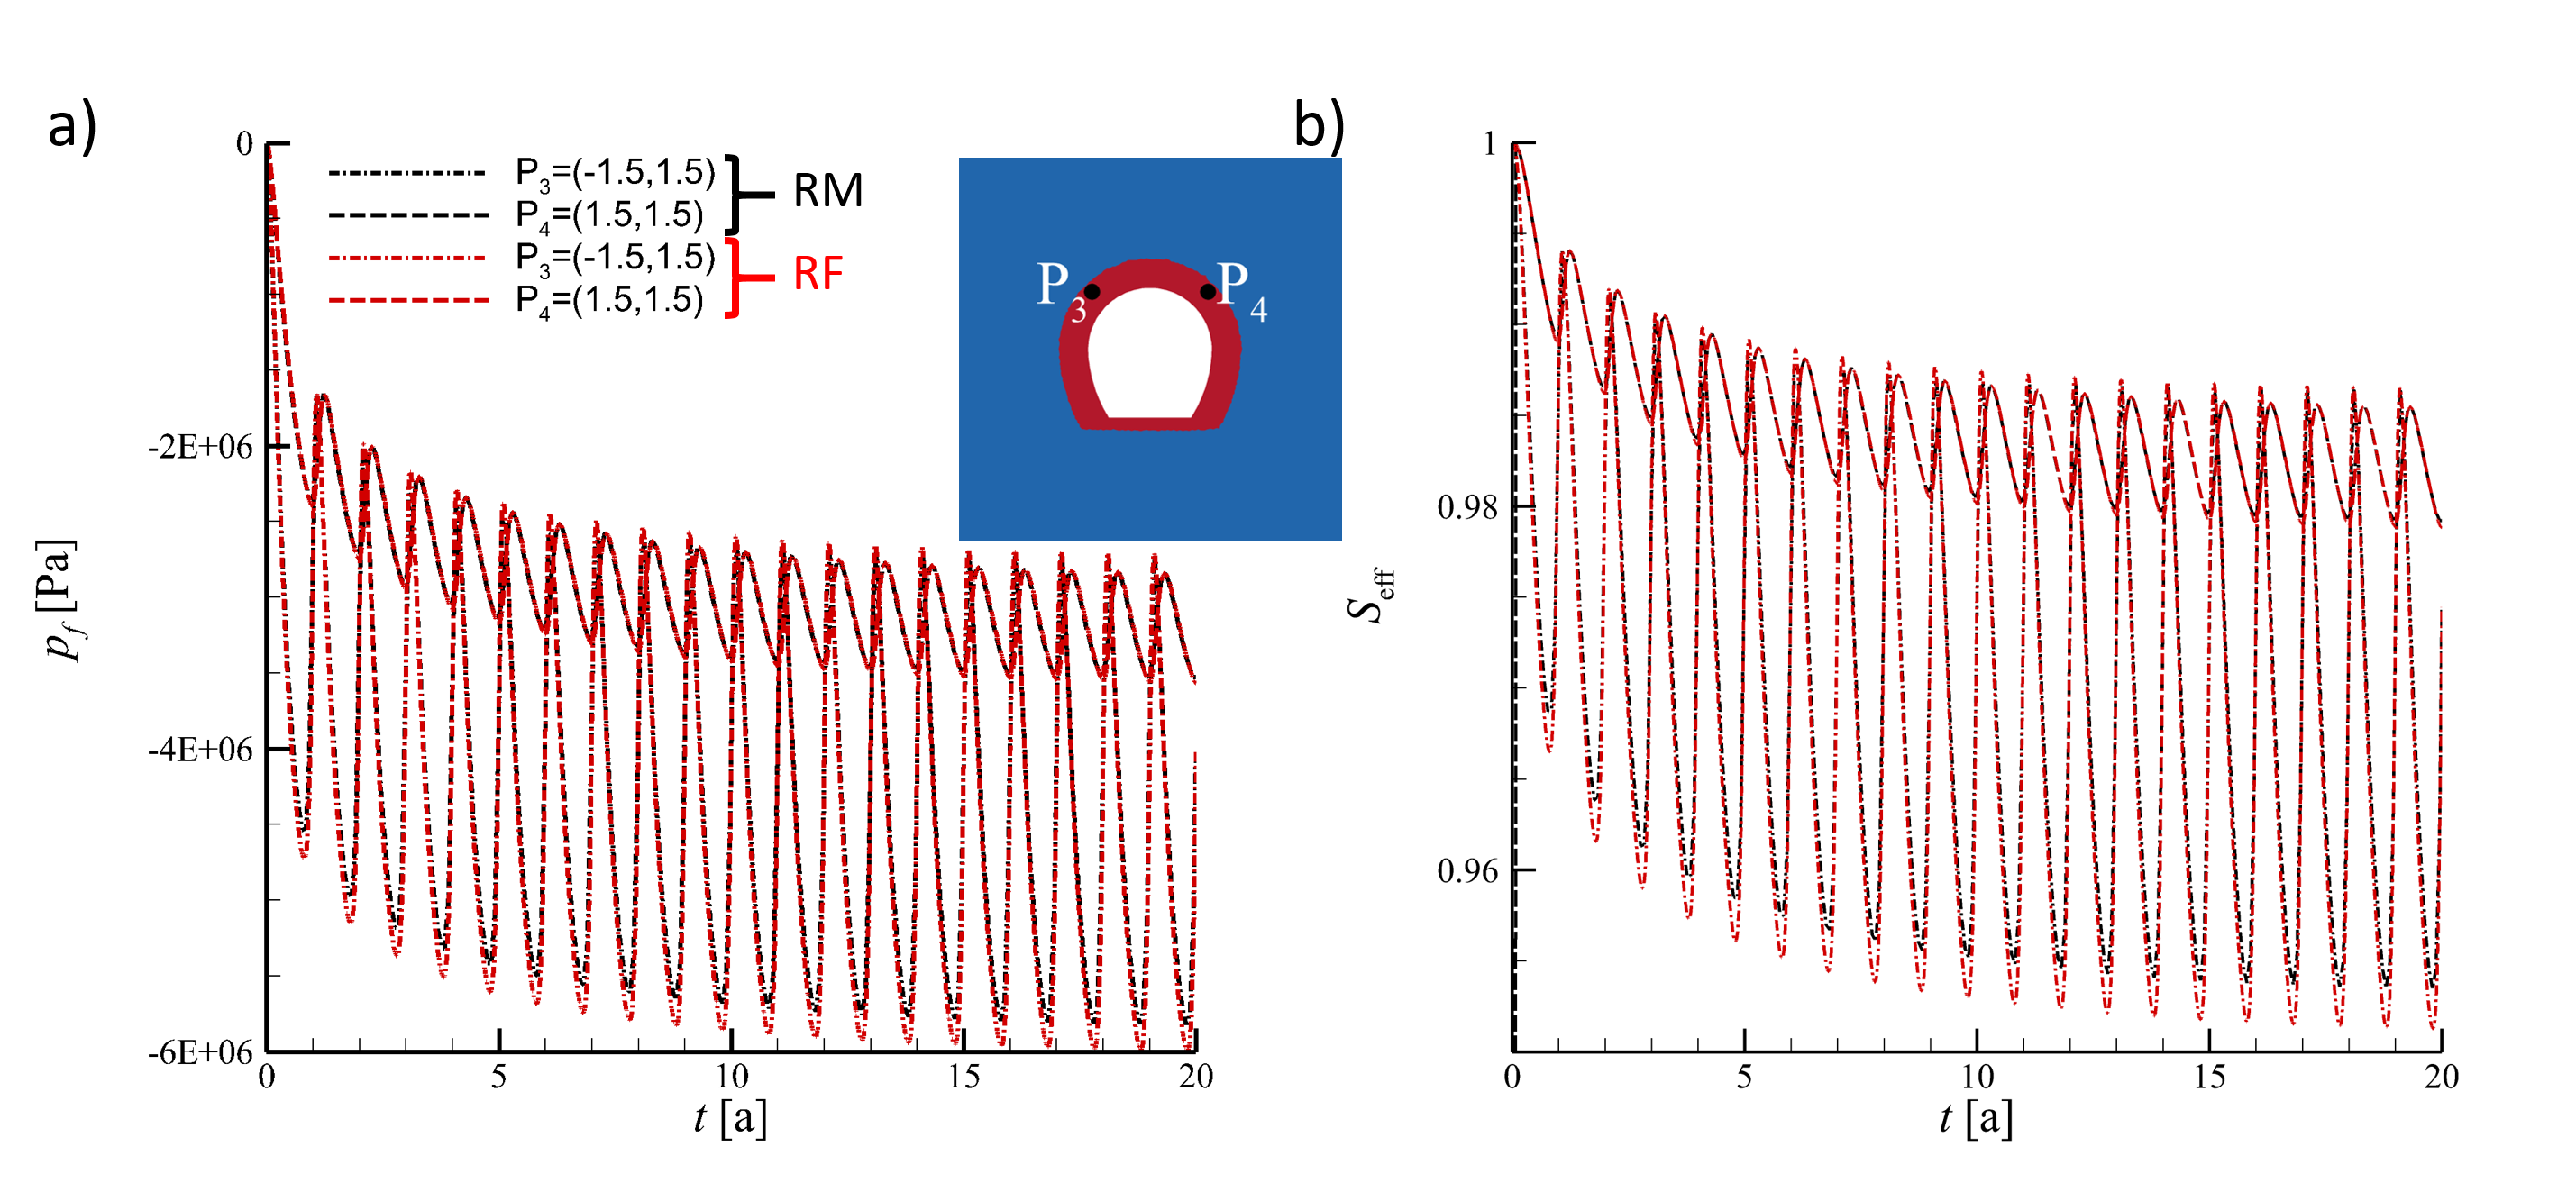
\includegraphics[width=\textwidth]{./figures/MEX10_cf_RF_RM.png}
\caption{Physical quantities probed over time at two characteristic locations for the model approaches 'Richards Flow' (RF, black) and 'Richards Mechanics' (RM, red). a) Fluid pressure and b) effective saturation. The inset shows the location of the sampling points relative to the niche.}
\label{fig:probe_RM_RF}
\end{figure}

\begin{figure}[t]
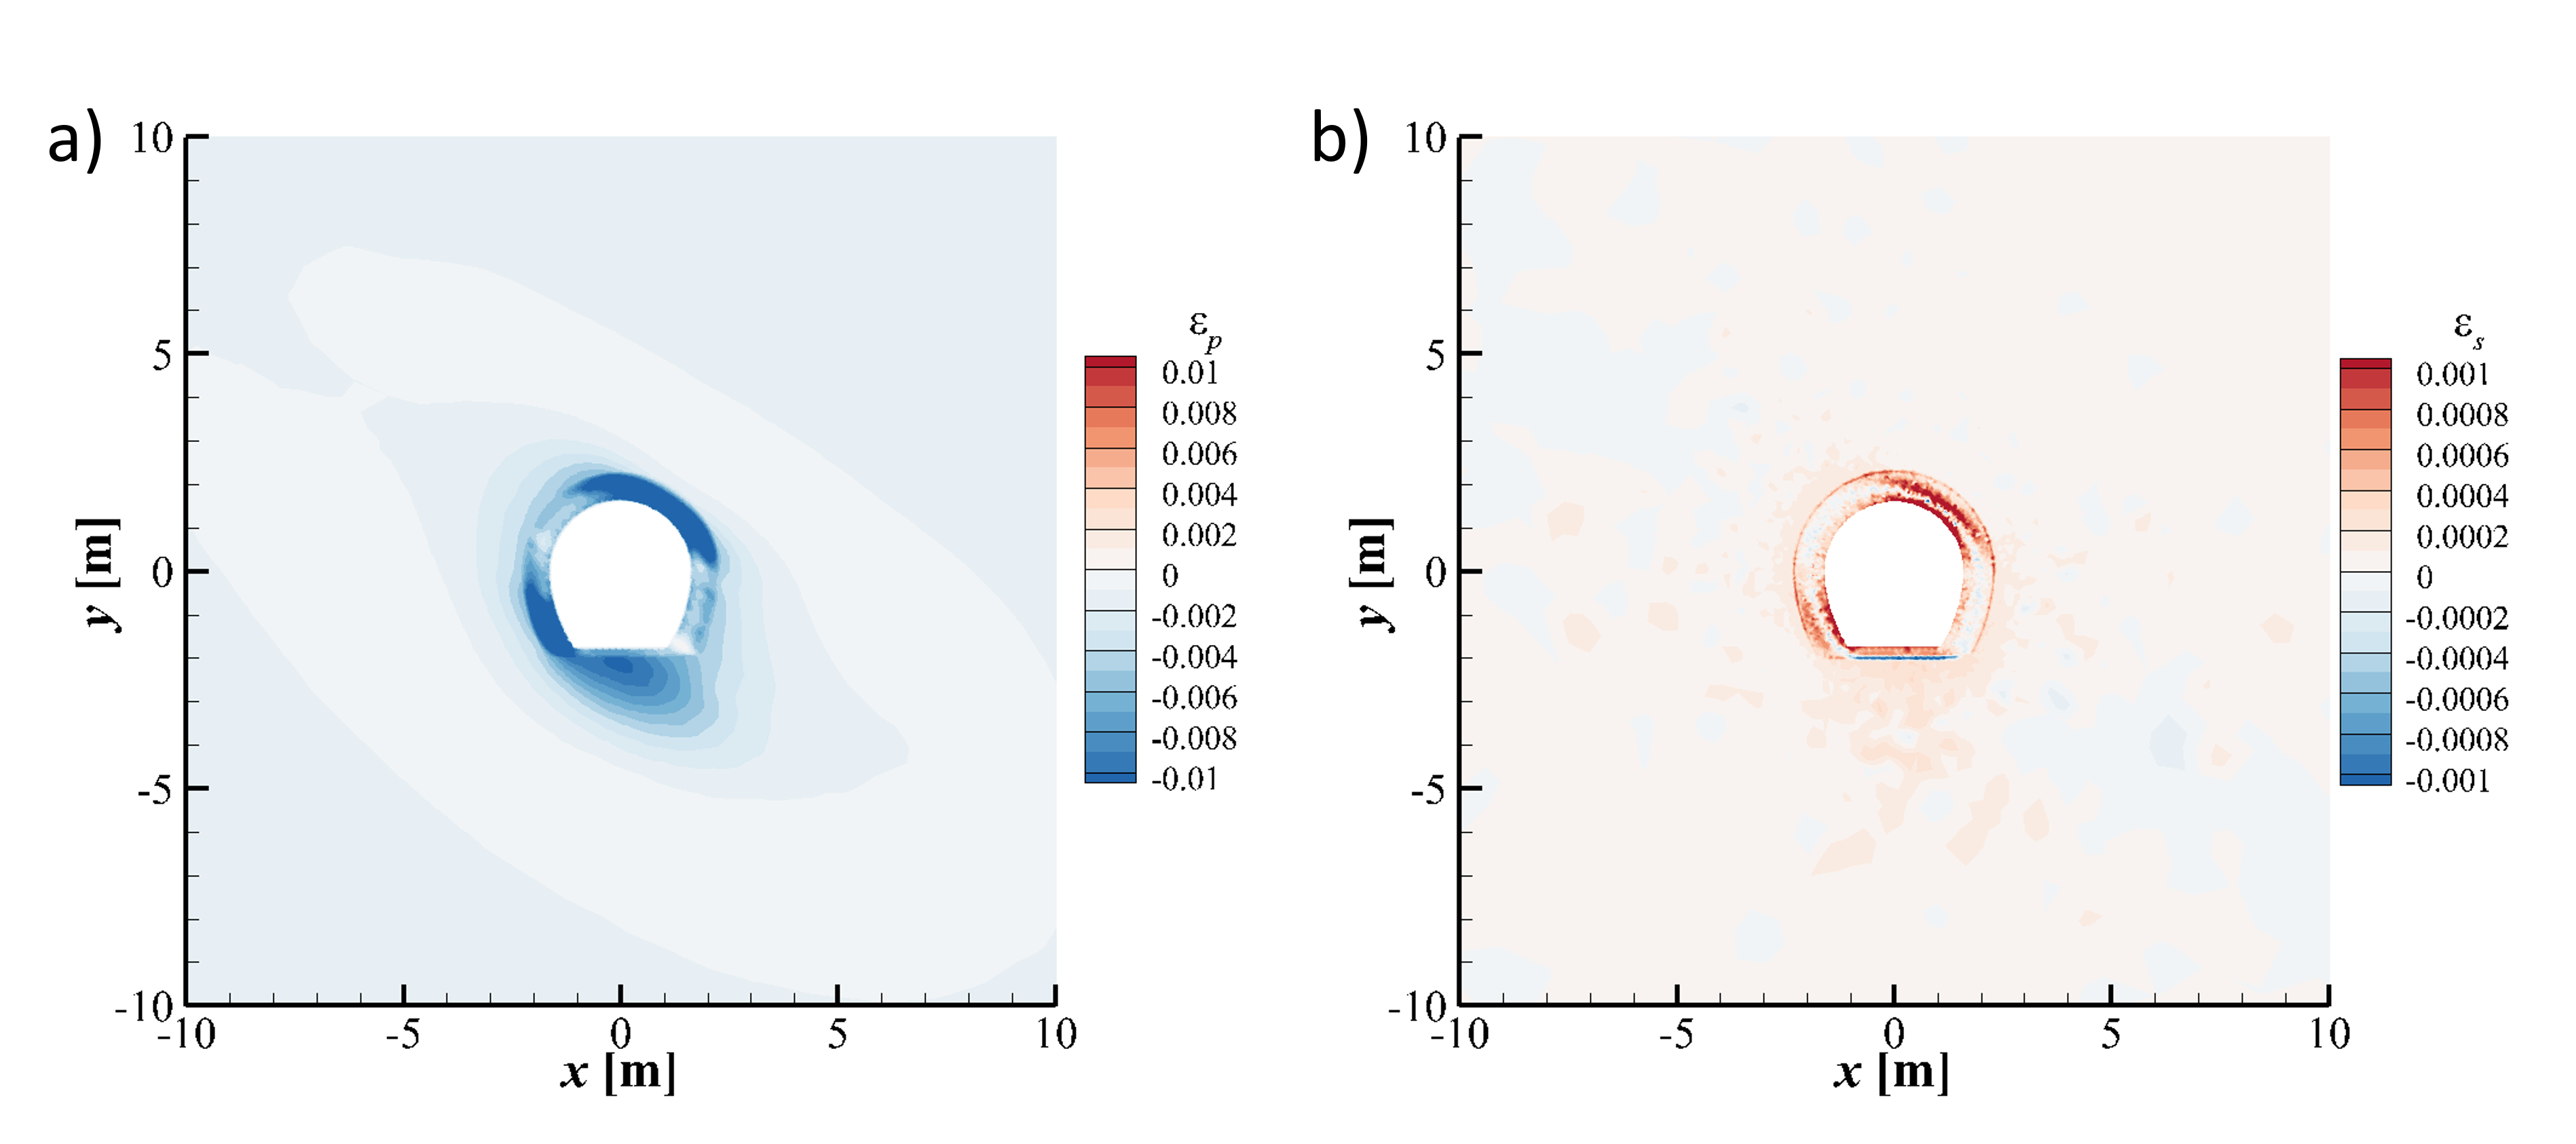
\includegraphics[width=\textwidth, trim=0.5cm  0.0cm 0 0.0cm, clip]{./figures/MEX10_cf_RF_RM_2d.png}
\caption{Deviation between 'Richards Flow' and 'Richards Mechanics' after 20 years of simulation time. a) Fluid pressure and b) effective saturation.}
\label{fig:richards_mechancis}
\end{figure}

The results of this comparison are shown in Figures \ref{fig:probe_RM_RF} and \ref{fig:richards_mechancis} as well as in Table \ref{tab:richards_mechanics}. For two sampling locations, the evolution of pressure and saturation show very good agreement. Note that the sampling locations for the data shown in Figure \ref{fig:probe_RM_RF} were taken inside the EDZ, since Figure \ref{fig:richards_mechancis} suggests that this is the area, where the strongest deviations can be expected. Indeed, while the cyclic saturation/desaturation is reproduced very well, there are differences in the maxima and minima between the two models for both quantities, $p_f$ and $S_\text{eff}$.  

Similar to the comparison made in Section \ref{sec:mex10_ogs5_vs_ogs6}, we define the simulation results reproduced by the RF model as the reference to compute the error
%
\begin{equation}\label{eq:error_rm_rf}
\epsilon_\theta = \frac{\theta^{RF}-\theta^{RM}}{\theta^{RF}}
\end{equation}
% 
as a quantitative estimate of the differences in the results of the two models. Looking at the two-dimensional deviations (Figure \ref{fig:richards_mechancis}), it becomes immediately obvious that pressure is slightly underestimated by the RM model in comaprison with the RF model within the EDZ (which yields that saturation is overestimated). The differences between the results computed by the algorithms of the two models is one order of magnitude larger compared to the analysis performed in Section \ref{sec:mex10_ogs5_vs_ogs6}. Especially the pressure shows higher deviations (Figure \ref{fig:richards_mechancis}a) at the transition between the EDZ and the undisturbed rock and at the walls of the niche. Nevertheless, the results computed by the two models are overall very similar. The RMSE of the simulation results remains far below 1\% (Table \ref{tab:richards_mechanics}). Hence, the implementation of the Richards equation into the model "Richards Mechanics" can be accepted as trustworthy for the present scenario. 

\begin{table}
 \caption{Deviations observed when comparing 'Richars Flow' with 'Richards Mechanics' in OGS-6.\label{tab:richards_mechanics}}
\begin{center}
\begin{tabular}{ l | c | c | c }
 Quantity			& Minimum 	& Maximum	 & RMSE  \\
 \hline
 $p_f$ & -0.0505 	& 0.0055	& $8.56\cdot 10^{-4}$\\ 
 $S_\text{eff}$	 	& -0.0405 & 0.0112	& $2.66\cdot 10^{-3}$\\		
\end{tabular}
\end{center}
\end{table}


%%%%%%%%%%%%%%%%%%%%%%%%%%%%%%%%%%%%%%%%%%%%%%%%%%%%%%%%%%%%%%%%%%%%%%%%%%%%%%%%%%%%%%%%%
\subsubsection{Comparison of OGS-5 and OGS-6 for the full "Richards Mechanics"-model}\label{sec:full_RM}
%%%%%%%%%%%%%%%%%%%%%%%%%%%%%%%%%%%%%%%%%%%%%%%%%%%%%%%%%%%%%%%%%%%%%%%%%%%%%%%%%%%%%%%%%
For the analysis presented in this section, we use the exact same hydraulic model and the computational setup as described in Section \ref{sec:model_RF}. Furthermore, we parameterize the mechanical model, which was summarized in Section \ref{sec:model_RM} by choosing $\alpha_{Biot}=1.0$, and keep $K_f=K_s=1\cdot 10^{100}$ Pa to drive the storage term to zero. We define $\textbf{u}_0=0$ m, which is zero displacements for the initial conditions, and use roller boundary conditions at $x=-25$ m and $x=25$ m. We fix the domain at the bottom ($y=-25$ m) by defining $u_y\rvert_{y=-25\text{m}}=0$ m, but we leave the upper boundary to be completely frictionless in both, the $x$ and $y$ direction.

Finally, we need to parameterize the elasticity tensor $\mathds{C}$, which is a function of the Young's modulus $E$ and Poissons' ratio $\nu$, where, again, we distinguish between undisturbed rock ($E_1$) and the EDZ ($E_2$). The parameterization of $\mathds{C}$, however, is conceptually different for isotropic and transverse isotropic conditions, since one can use different definitions depending on the simplicity/symmetry of the problem. Since we are investigating both conditions, these definitions will be detailed below. The transverse isotropic condition is known to be more adequate for clayrock owing to the bedding of this particular rock and it was also used in the study of \cite{ziefle2018}.

\subsubsection*{Isotropic elasticity}
As mentioned above, we use the Voigt notation to write the three-dimensional elasticity tensor. For isotropic conditions, $\mathds{C}$ simplifies from the general form to
\begin{equation}
\mathds{C} =  \frac{E}{(1+\nu)(1-2\nu)}	
				\begin{pmatrix}
				1-\nu 	& \nu	& \nu	& 0				   &0					&0 	\\
				\nu	  	& 1-\nu	& \nu	& 0				   &0					&0	\\
				\nu		& \nu	& 1-\nu	& 0				   &0					&0	\\		
				0		& 0		& 0		& \frac{1-2\nu}{2} &0					&0	\\		
				0		& 0		& 0		&0				   &\frac{1-2\nu}{2}	&0	\\		
				0		& 0		& 0		&0				   &0      &\frac{1-2\nu}{2}
				\end {pmatrix}
\end{equation}
Hence, $\mathds{C}$ is fully parameterized with $\nu=0.18$ for both material groups, $E_1=3.6 \times 10^9$ Pa for the undisturbed rock and $E_2=1.8\times 10^9 $ Pa for the EDZ.


While the simulation results of the RM-model yield very similar spatial distributions of $p_f$ and $S_\text{eff}$ that were reported in Figure \ref{fig:results}, we know obtain values for the deformation vector $\textbf{u}$. The results for the two components after a simulation time of 20 years is shown in Figure \ref{fig:RM_displacement_isotropic}. The overall impact of the saturation/desaturation on the mechanical behavior is such that the tunnel is compressed in its height, whereas the lateral distance between the walls increases. This deformation leads to a compression in the undisturbed rock farther away from the niche.  

\begin{figure}[t]
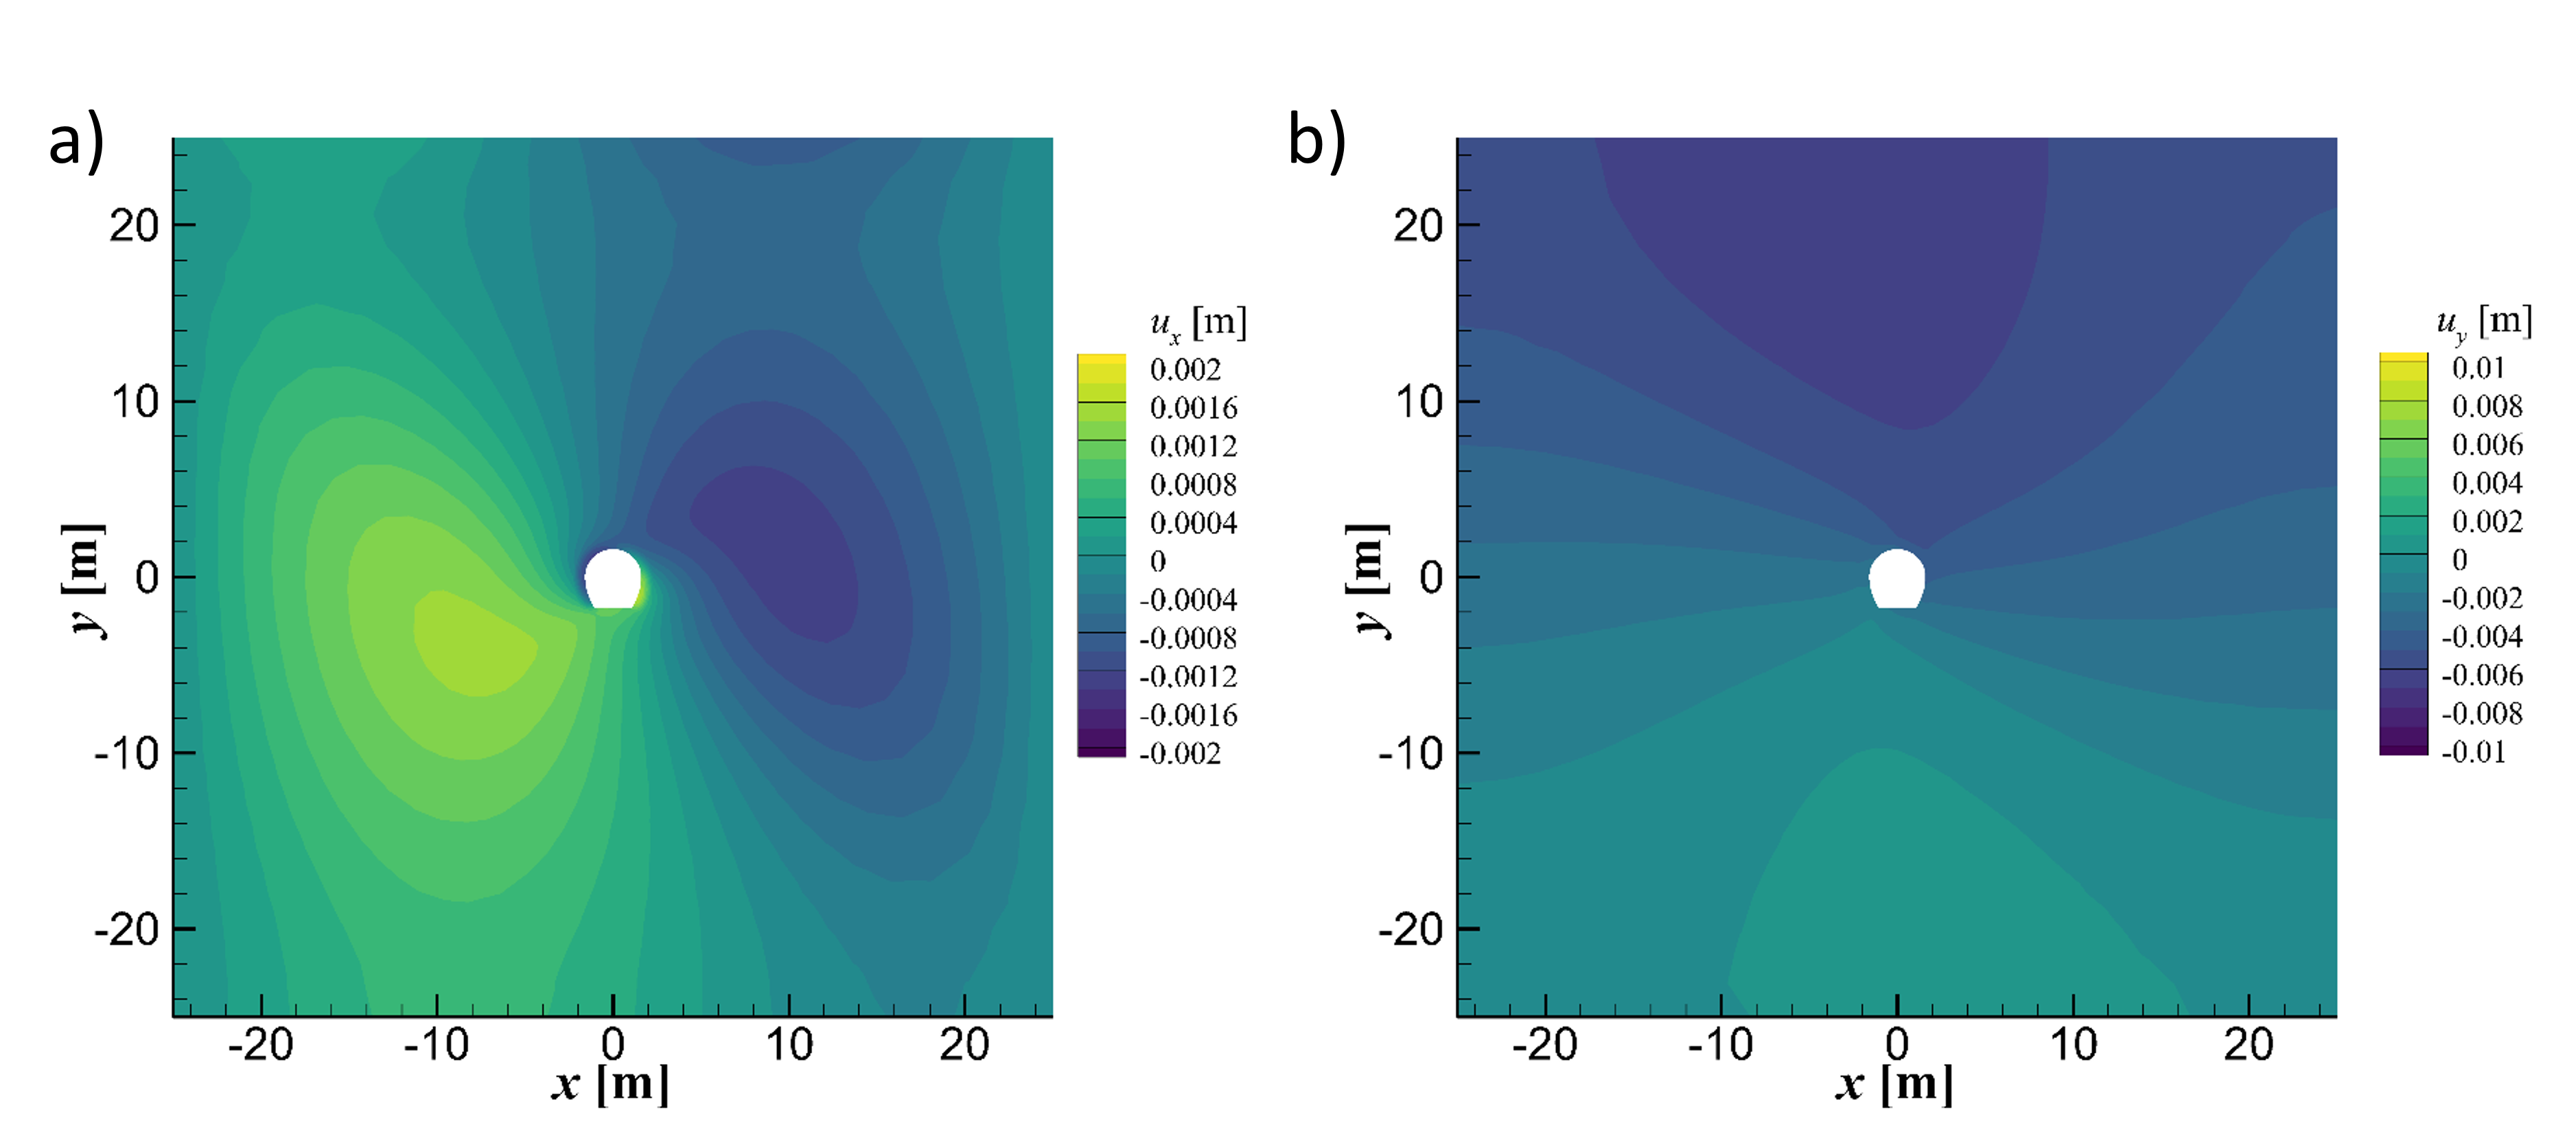
\includegraphics[width=\textwidth, trim=0.5cm  0.0cm 0 0.0cm, clip]{./figures/MEX10_RM_OGS5_isotropic.png}
\caption{Spatial distribution of the rock deformation $\textbf{u}$  for isotropic conditions after 20 years of simulation time. a) horizontal deformation $u_x$ and b) vertical deformation $u_y$.}
\label{fig:RM_displacement_isotropic}
\end{figure}

\begin{figure}[t]
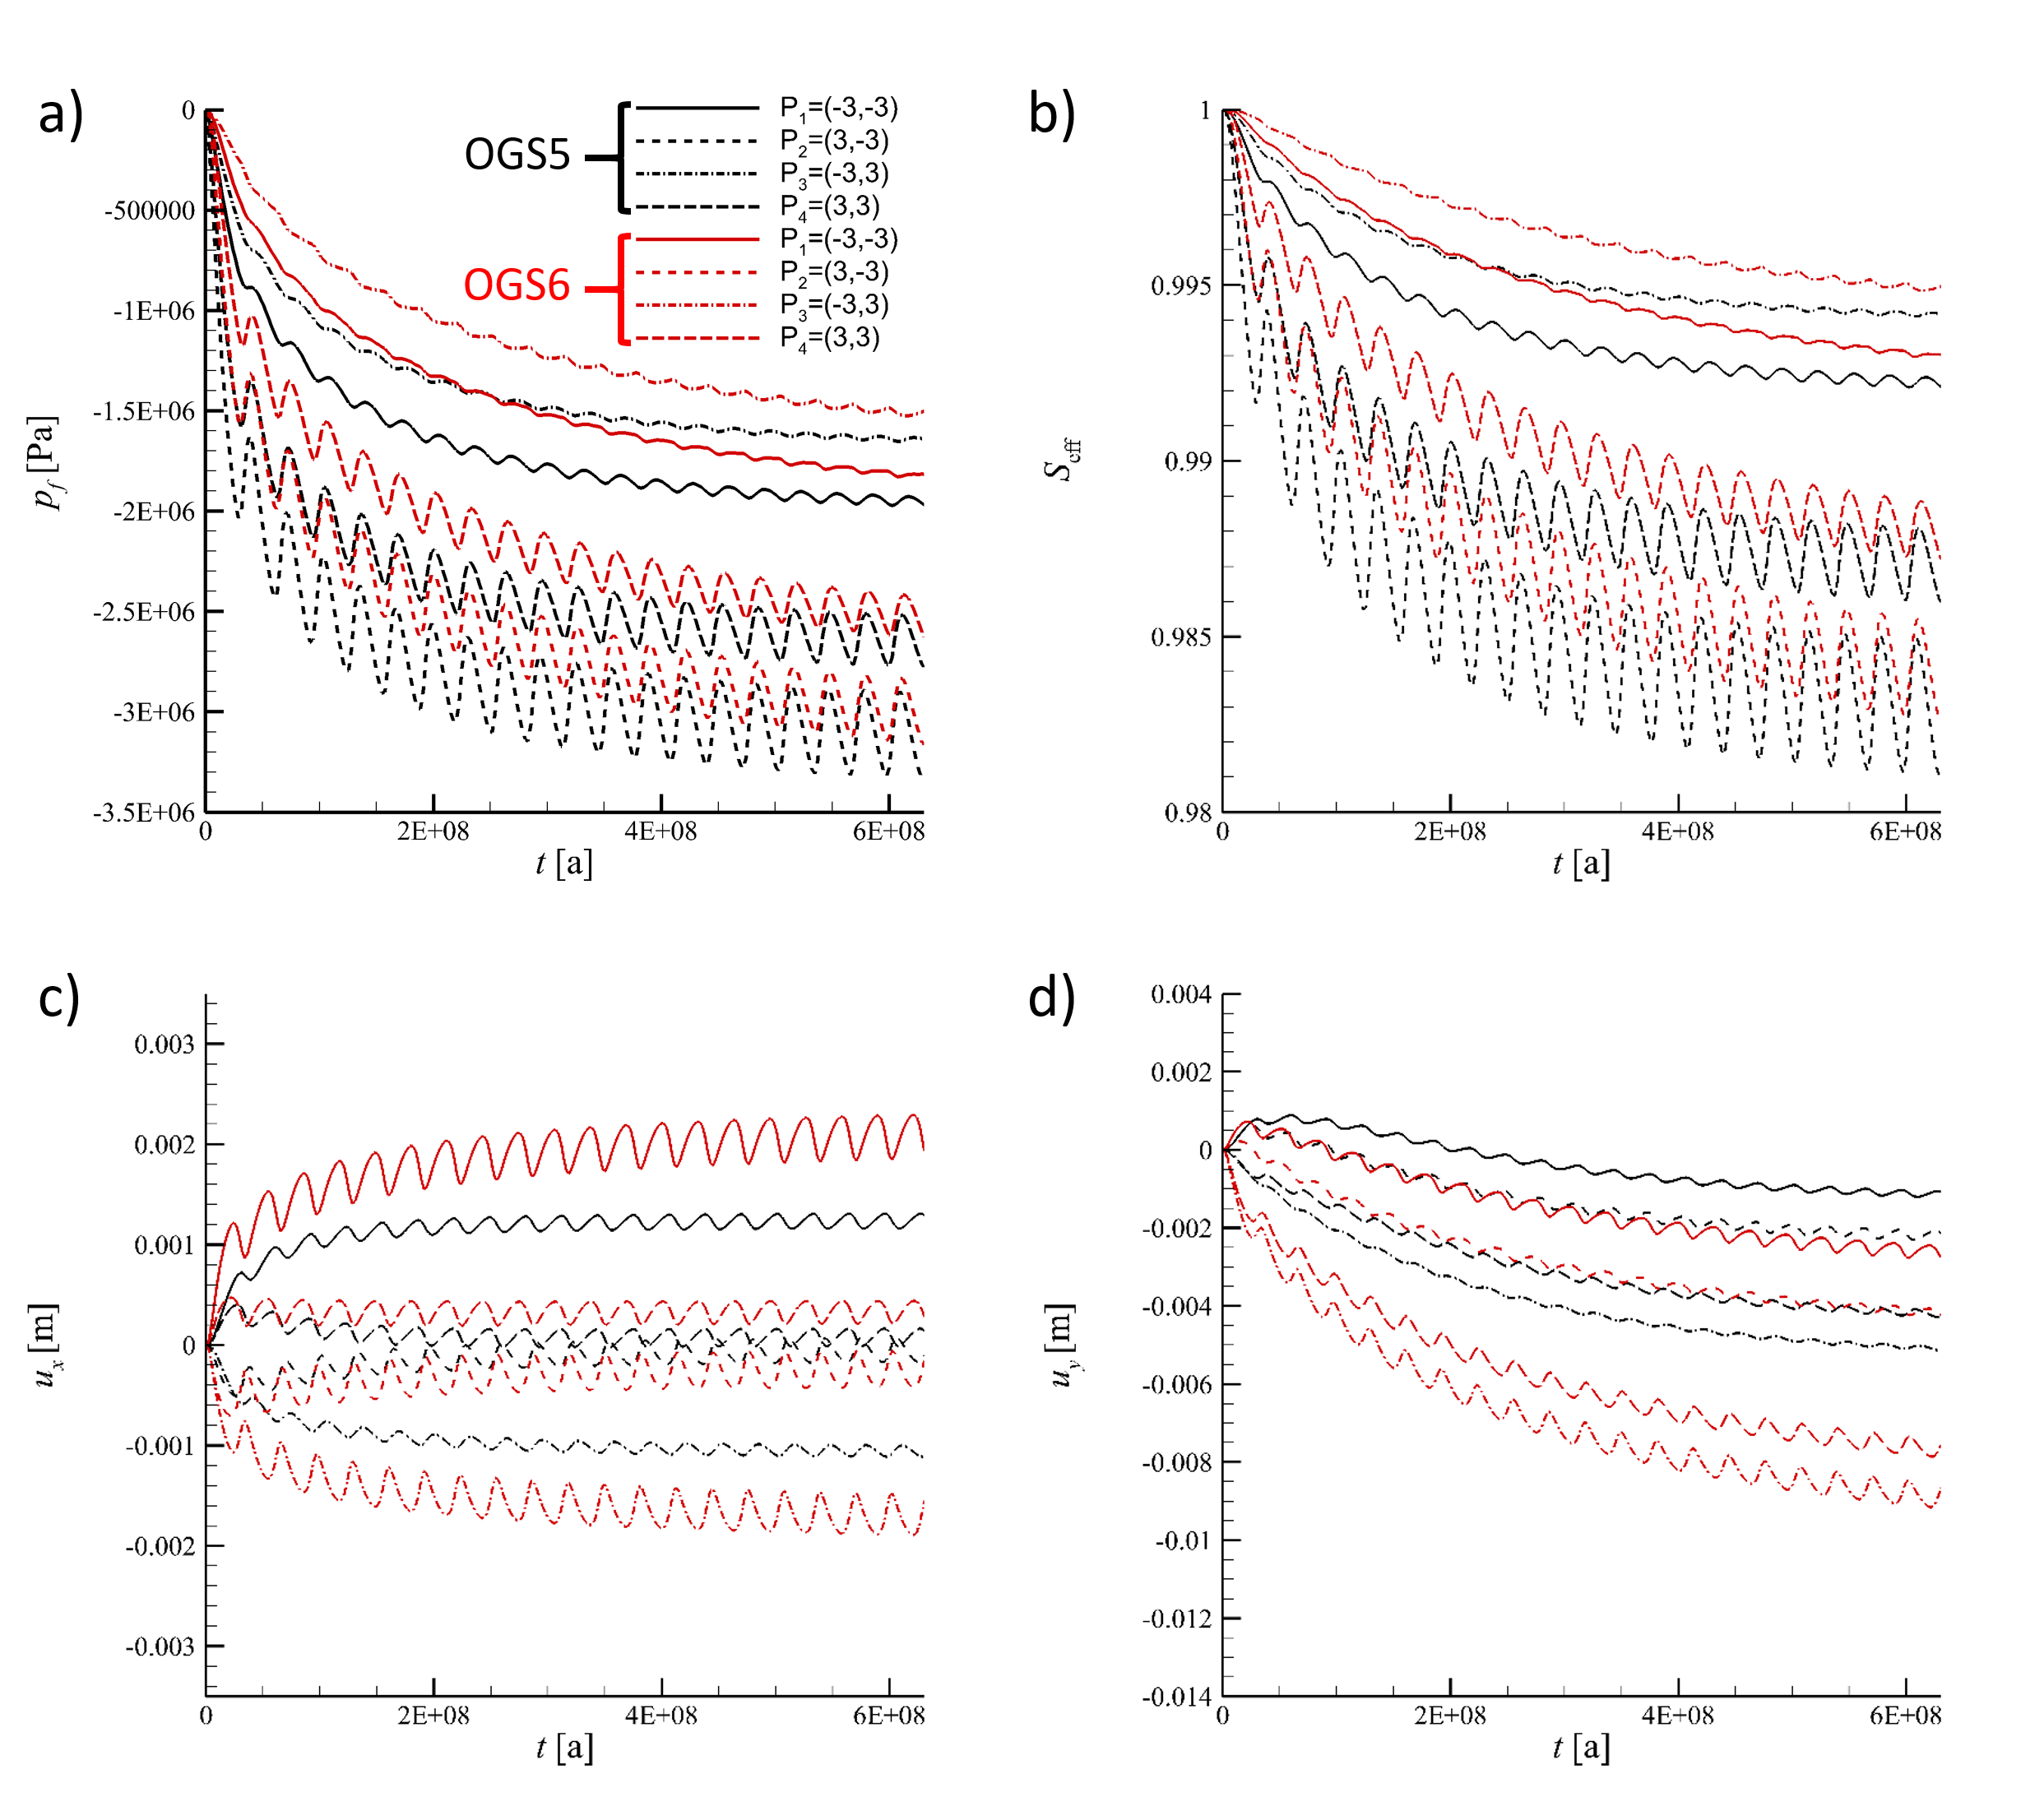
\includegraphics[width=\textwidth, trim=0.5cm  0.0cm 0 0.0cm, clip]{./figures/MEX10_probe_over_time_isotropic.png}
\caption{Physical quantities computed by OGS-5 and OGS-6 for isotropic conditions probed over time at the same four locations depicted in the inset of Figure \ref{fig:cf_P_S}. a) Fluid pressure, b) effective saturation, c) horizontal deformation and d) vertical deformation.}
\label{fig:RM_probe_over_time_isotropic}
\end{figure}

To compare the simulation results of the two FE codes OGS-5 and OGS-6, we probe the generated data of $p_f$, $S_\text{eff}$, $u_x$ and $u_y$ over time at the sampling points illustrated in the inset of Figure \ref{fig:cf_P_S}. Unlike the very good agreement obtained in that figure, we now find significant deviations between the simulation results of OGS-5 and OGS-6. This is true for all physical quantities at all sampling points. We obtain a systematically higher pressure and, hence, a higher saturation for OGS-6. This difference also causes different mechanical deformations of the rock, but these quantities do not differ as systematic as the pressure does. The difference can be explained by the different coupling schemes of the two codes. While OGS-5 uses a staggered scheme with a weak coupling of the two processes, OGS-6 provides a monolithic scheme that allows for a strong coupling of the hydraulic and mechanical processes by solving for $p_f$ and $\textbf{u}$ simultaneously. The strongly coupled monolithic scheme is known to yield better results than the weakly coupled staggered scheme \cite{hubner2003,farhat2000}. Hence, the simulation results generated by OGS-6 potentially provide more realistic results than OGS-5 does. However, a detailed comparison to analytic reference solutions or experimental benchmark data will be needed to verify this hypothesis.


Despite the differences of the results reported in Figure \ref{fig:RM_probe_over_time_isotropic}, both simulations yield qualitatively the same results, albeit with different magnitudes in deformation. This becomes evident in the spatial distribution of the error \eqref{eq:error}, which is shown in Figure \ref{fig:RM_error_2d_isotropic}. Note that values of $\epsilon_{u,x}$ and $\epsilon_{u,y}$ were normalized by the width of the niche, which is 3.2 m, rather than $\epsilon^{OGS5}$, as normalizing by the small deformation values is prone to indicate unreasonably large errors. Even though there is a direct dependency of effective saturation on fluid pressure, the spatial distributions of the relative error for these two quantities look very differently (Figure \ref{fig:RM_error_2d_isotropic}a and b). The rather large error for fluid pressure especially far away from the niche can be attributed to low values of $p_f$ that are used to normalize \eqref{eq:error_rm_rf}. Closer to the niche, the error decays to smaller values. Looking at the spatial distribution of the error for all other quantities, however, we can conclude that even though the coupling scheme of OGS-6 is more powerful than the scheme of OGS-5, both simulations yield similar results. This fact is also reflect in the maxima, minima and RMSE \eqref{eq:RMSE}. Even though the deviations in pressure are rather large, the overall change in deformation with respect to the characteristic length of the problem, i.e. the width of the niche, remains small. Nevertheless, unlike the comparison presented in Section \ref{sec:model_RF}, we observe substantial deviations for the simulation results from OGS-6 compared to those generated using OGS-5. Further research will be needed to clarify these differences. 

\begin{figure}[t]
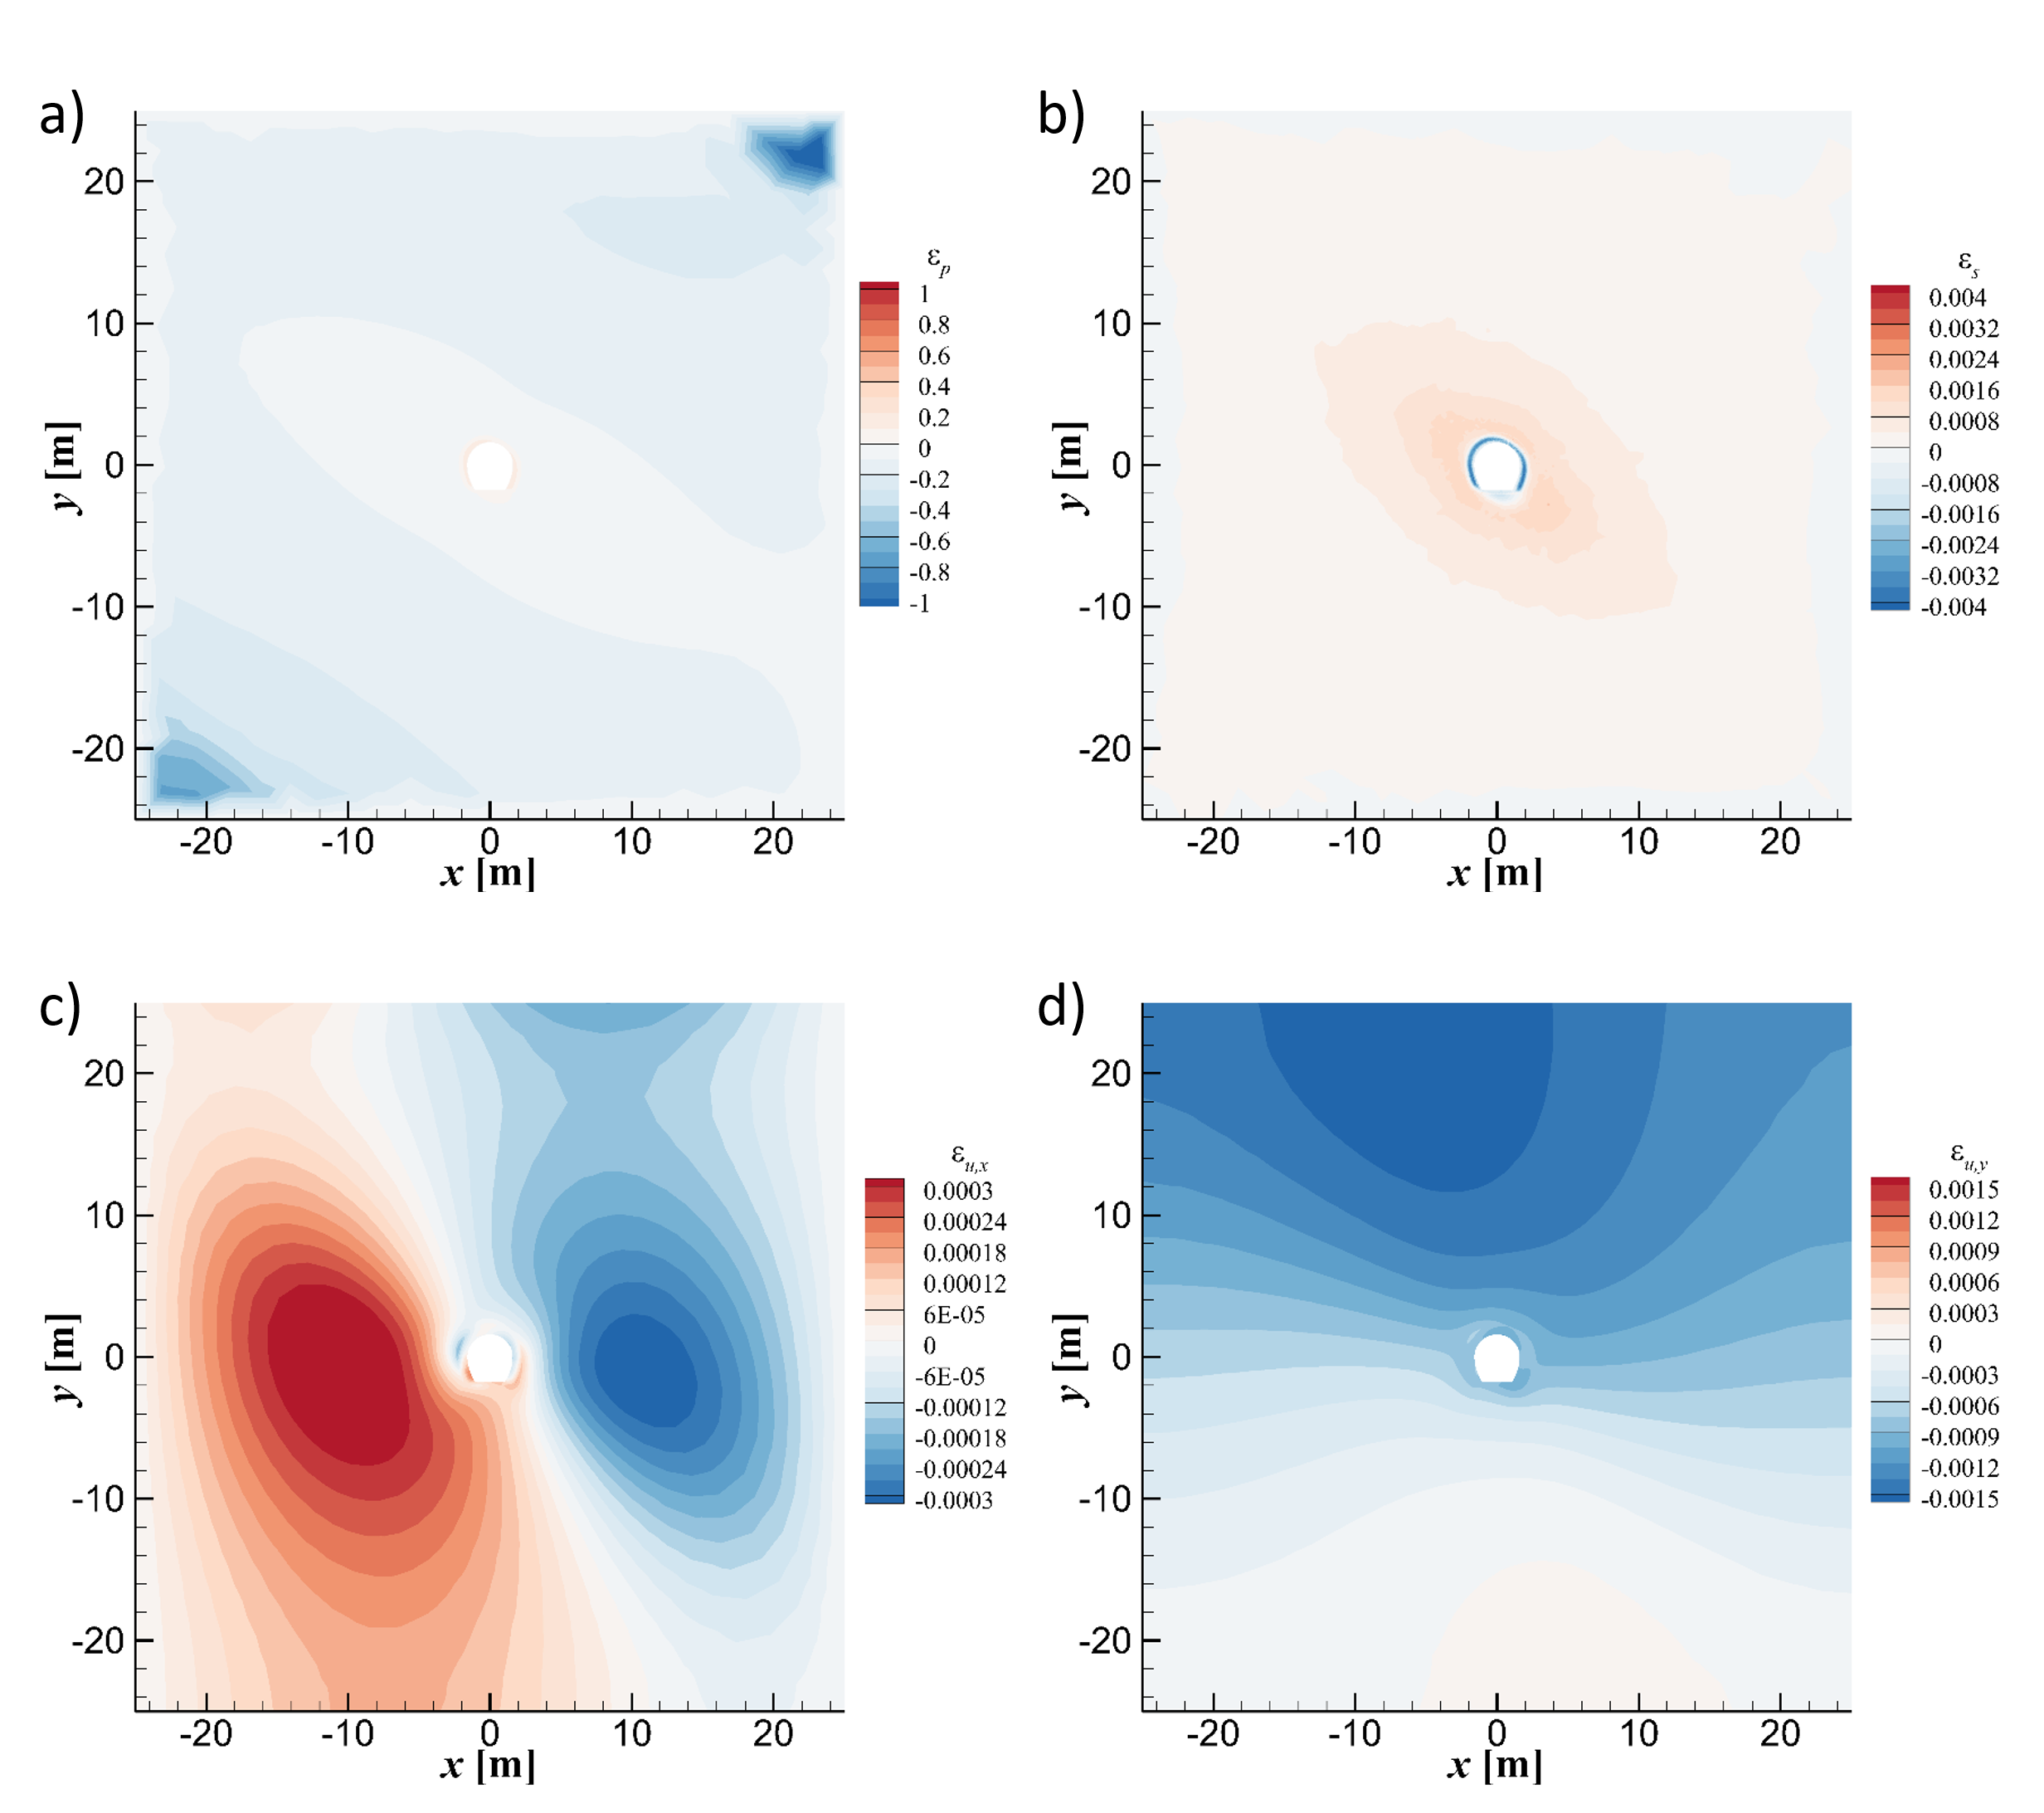
\includegraphics[width=\textwidth, trim=0.5cm  0.0cm 0 0.0cm, clip]{./figures/MEX10_RM_error_2d_isotropic.png}
\caption{Deviations between OGS-5 and OGS-6 for isotropic conditions after 20 years of simulation time.  a) Fluid pressure, b) effective saturation, c) horizontal deformation and d) vertical deformation.}
\label{fig:RM_error_2d_isotropic}
\end{figure}

\begin{table}
 \caption{Deviations observed when comparing OGS-5 with OGS-6 for the RM model with isotropic conditions.\label{tab:error_RM_isotropic}}
\begin{center}
\begin{tabular}{ l | c | c | c }
 Quantity				& $\min{(\epsilon)}$ 	& $\max{(\epsilon)}$	 & RMSE  \\
 \hline
 $p_f$				& -1.1514 				& 0.1478 			& $6.81\cdot 10^{-2}$\\ 
 $S_\text{eff}$	 	& -0.0045 				& 0.0017			& $1.12\cdot 10^{-3}$\\		
 $u_x$				& -0.0003 				& 0.0004			& $8.97\cdot 10^{-5}$\\		 
 $u_y$			 	& -0.0016 				& $3\cdot10^{-5}$	& $8.44\cdot 10^{-4}$\\	
\end{tabular}
\end{center}
\end{table}

\subsubsection*{Anisotropic elasticity}
We consider the transverse isotropic behavior of clayrock described in Section \ref{sec:model_RF} by defining a higher stiffness parallel to the bedding $E_i$ and a lower stiffness normal to the bedding $E_a$. Here, the subscripts $i$ and $a$ indicate directions parallel and perpendicular to the bedding plane, respectively. Similarly, the Poisson's ratio has to be defined with respect to the anisotropy  direction that is normal to the bedding $\nu_{ia}$ and parallel to the bedding $\nu_{ii}$.  The inverse of the elasticity tensor then becomes
\begin{equation}
\mathds{C}^{-1} =  	\begin{pmatrix}
 	\frac{1}{E_i} 		& -\frac{\nu_{ai}}{E_a}	& -\frac{\nu_{ii}}{E_i}	& 0	&0	&0 	\\
	-\frac{\nu_{ia}}{E_i}&\frac{1}{E_a}			& -\frac{\nu_{ia}}{E_a}	& 0	&0	&0 	\\
	-\frac{\nu_{ii}}{E_i}& -\frac{\nu_{ai}}{E_a}	&\frac{1}{E_i}		& 0	&0	&0 	\\
				0		& 0		& 0		& \frac{1}{G_a} &0				&0			\\		
				0		& 0		& 0		&0				&\frac{1}{G_i}	&0			\\	
				0		& 0		& 0		&0				&0		      	&\frac{1}{G_a} 	
				\end {pmatrix}
\end{equation}
where $G_i=E_i/(2+2\nu_{ii})$ and $G_a$ are the shear moduli in isotropic and anisotropic direction, respectively. Note that the elasticity tensor is not symmetric. Instead, we need to rescale $\nu_{ai}=\nu_{ia} \frac{E_a}{E_i}$. Here, we have used the same values as \cite{ziefle2018}, which were $E_{i}=3.6\times10^9$ Pa, $E_{a}=1.1\times10^9$ Pa, $\nu_{ia}=0.16$ and $\nu_{ii}=0.18$ and  $G_a=1.2\times10^9$ Pa. We rotate the elasticity tensor by the same angle of inclination $\gamma = -32.96^{\circ}$ that was applied to the permeability tensor \eqref{eq:permeabilities}. 

\begin{figure}[t]
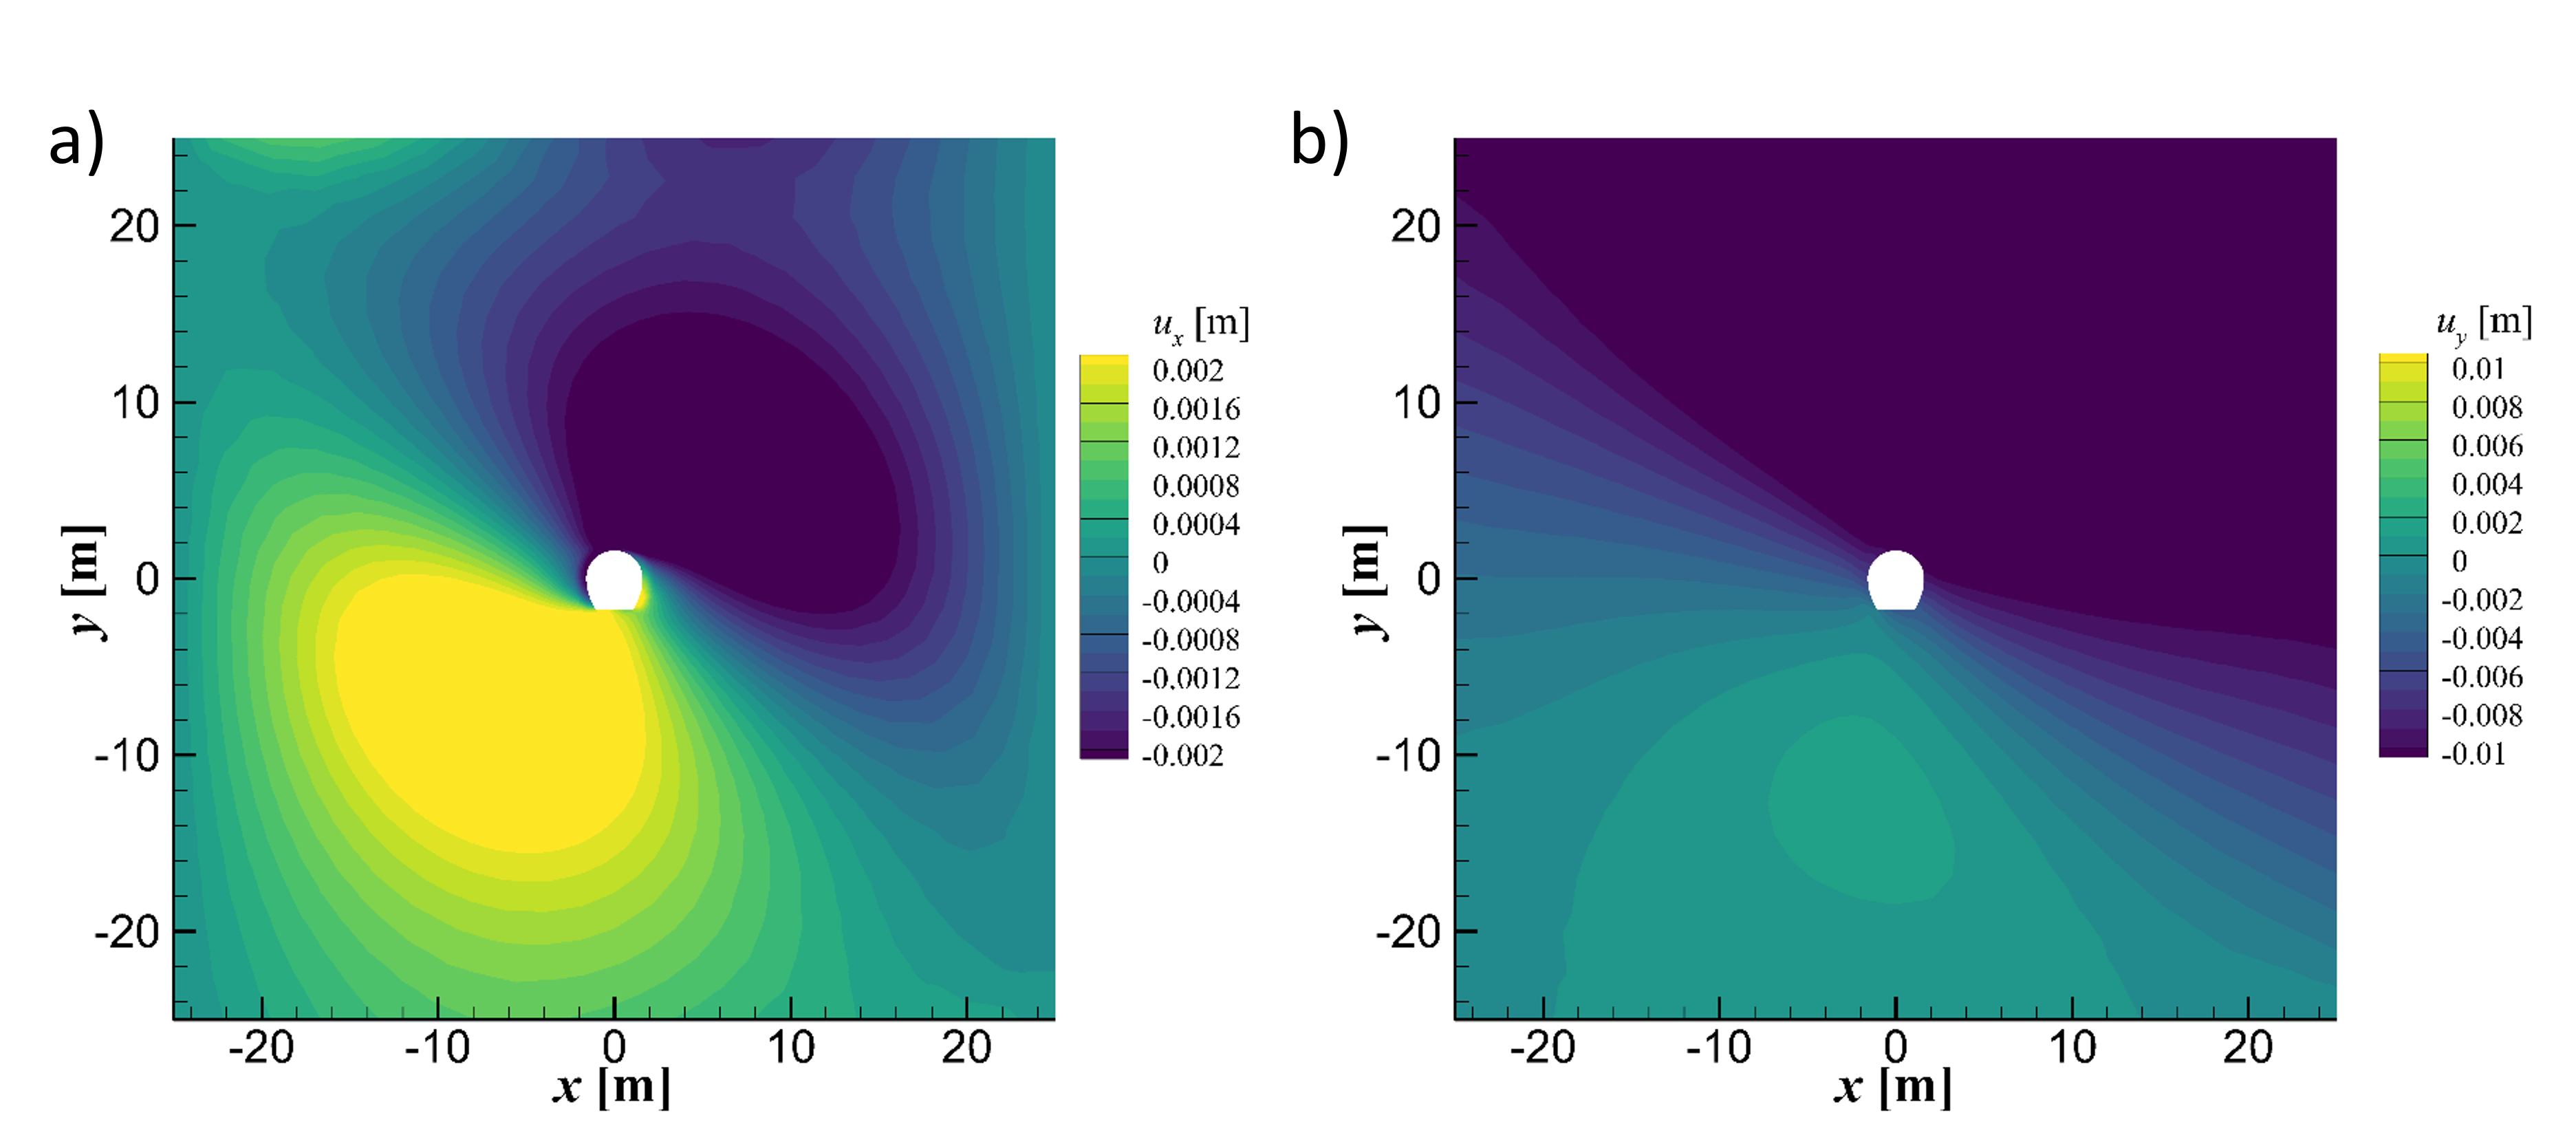
\includegraphics[width=\textwidth, trim=0.5cm  0.0cm 0 0.0cm, clip]{./figures/MEX10_RM_OGS5_anisotropic.png}
\caption{Spatial distribution of the rock deformation $\textbf{u}$  for anisotropic conditions after 20 years of simulation time. a) horizontal deformation $u_x$ and b) vertical deformation $u_y$.}
\label{fig:RM_displacement_anisotropic}
\end{figure}

To illustrate the well-developed stage and to provide a comparison to the isotropic elasticity shown in Figure \ref{fig:RM_displacement_isotropic}, we plot the spatial distribution of the two components of the deformation in Figure \ref{fig:RM_displacement_anisotropic}. As desired,the maximum and minimum horizontal deformations have rotated for the anisotropic case according to the angle of inclination. Other than that, the simulation results of the isotropic and anisotropic case  remain very similar.

\begin{figure}[t]
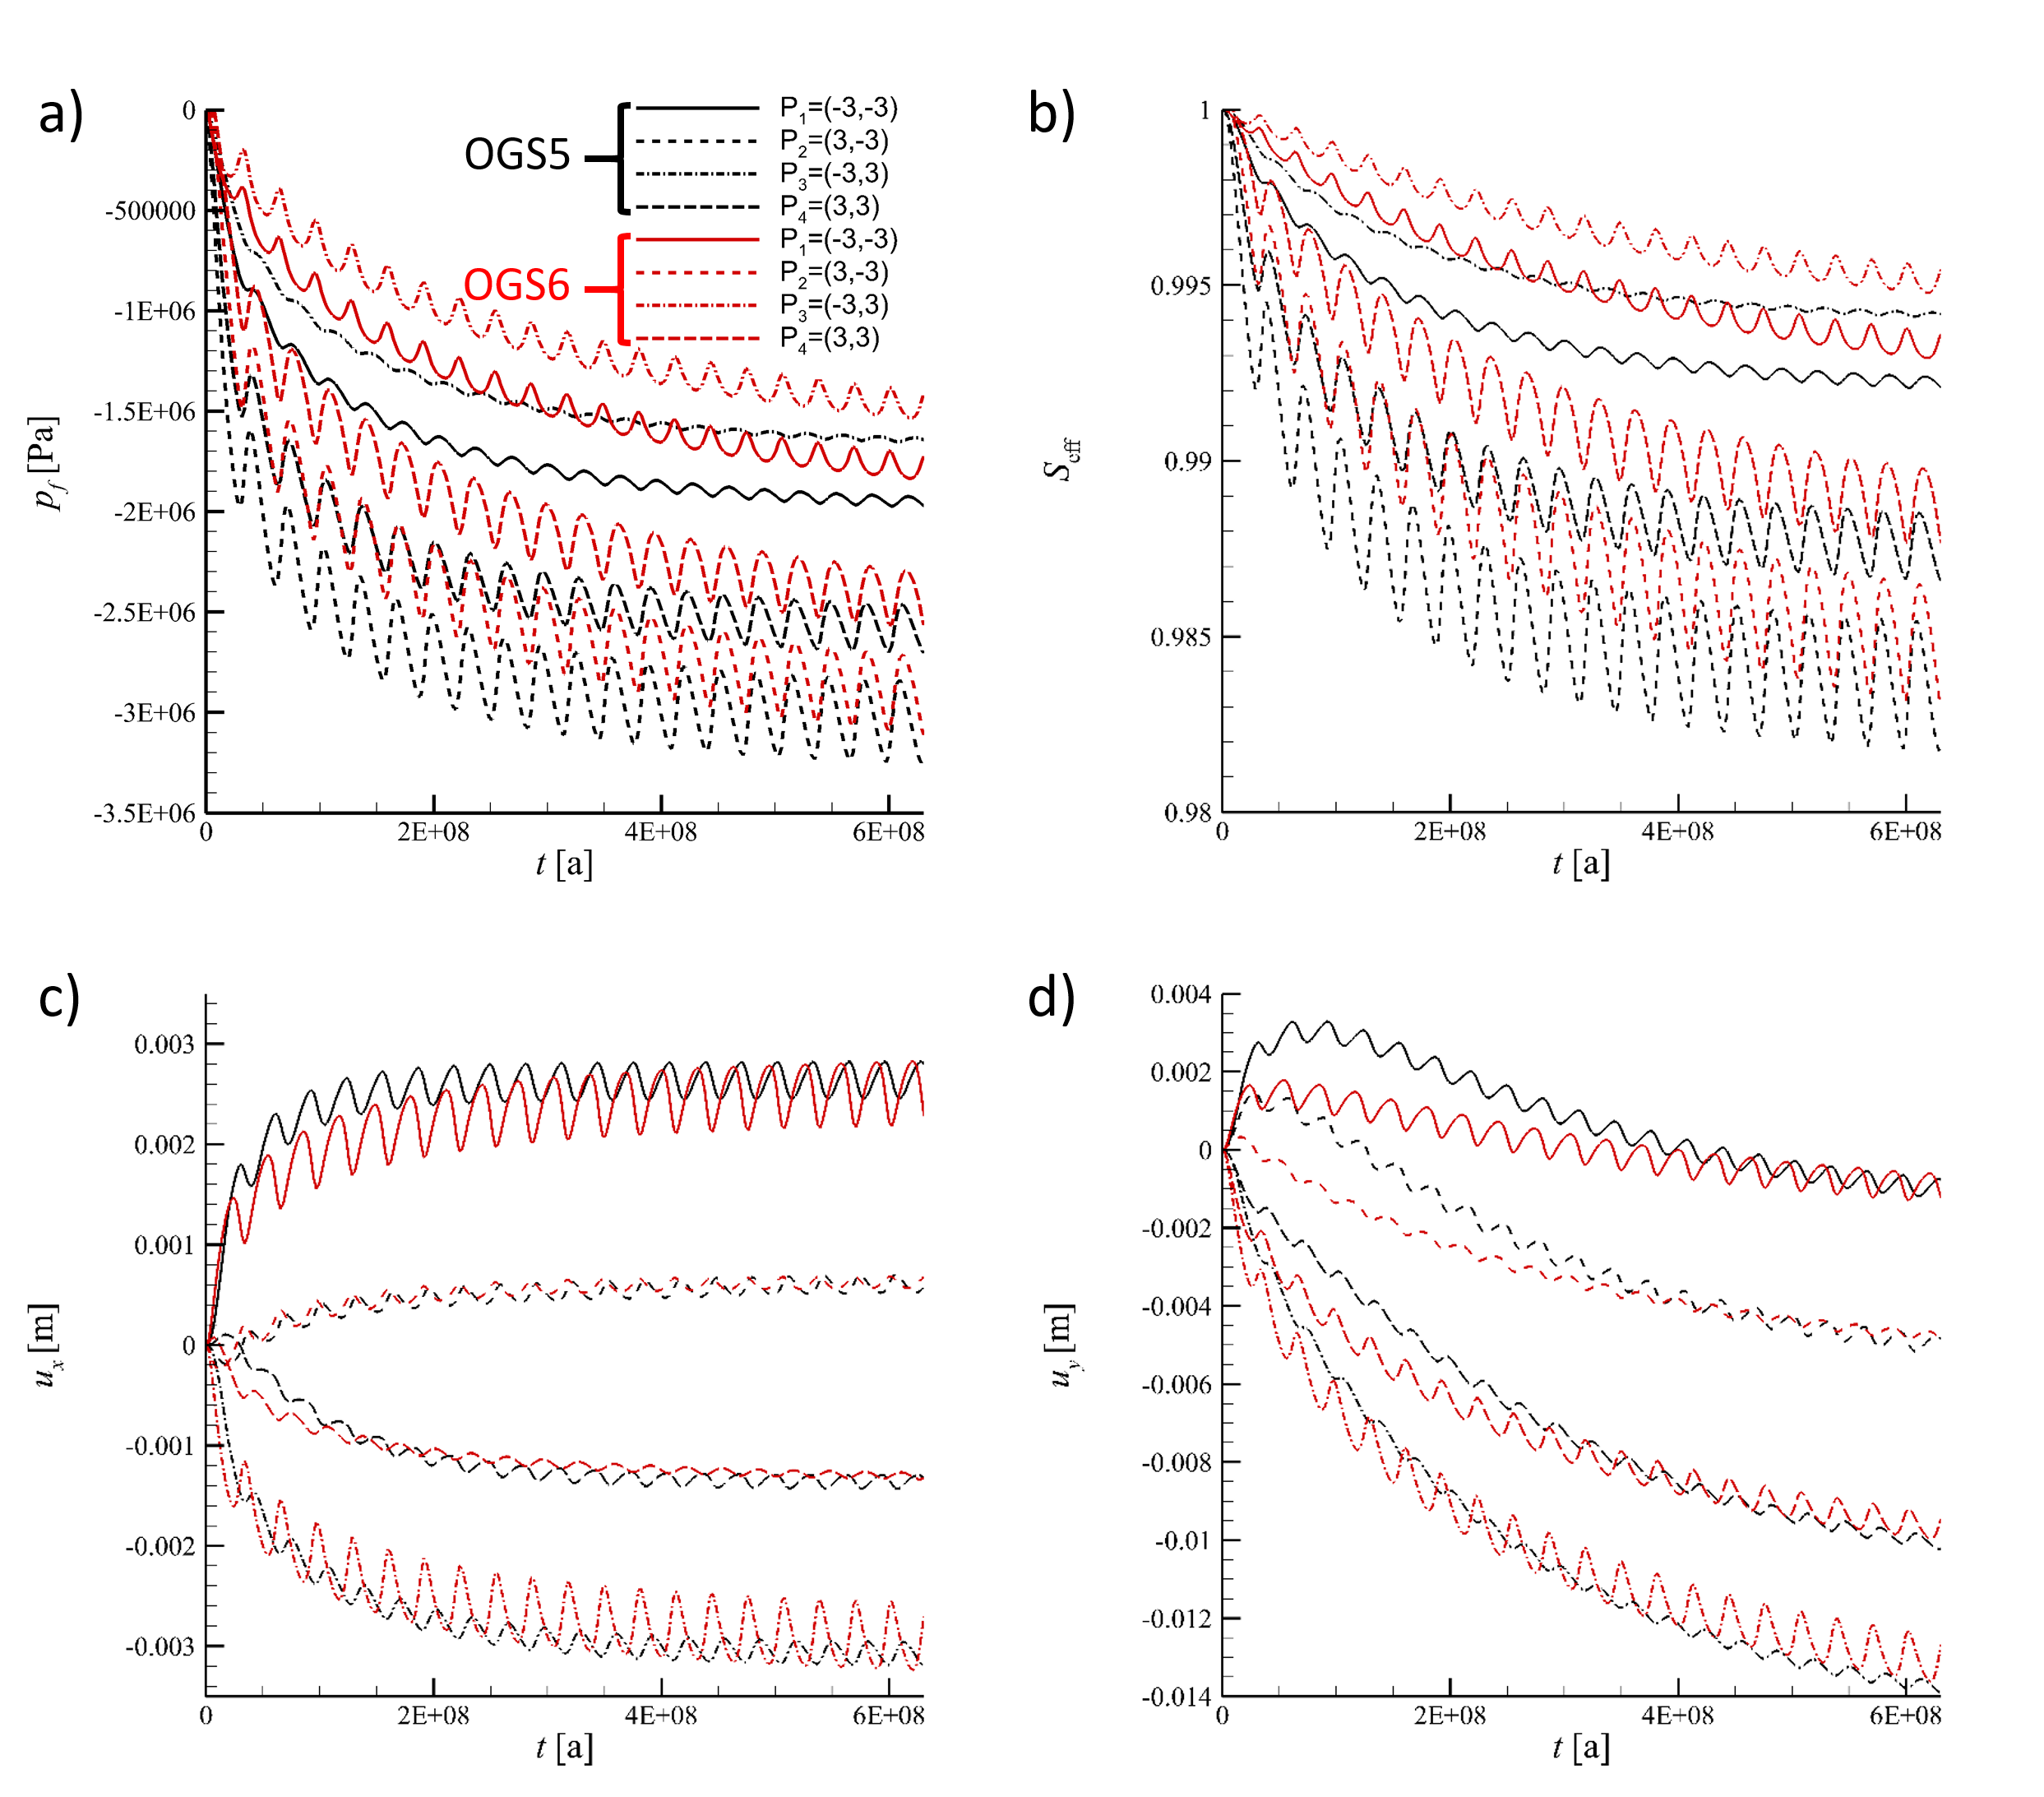
\includegraphics[width=\textwidth, trim=0.5cm  0.0cm 0 0.0cm, clip]{./figures/MEX10_probe_over_time_anisotropic.png}
\caption{Physical quantities computed by OGS-5 and OGS-6 for anisotropic conditions probed over time at the same four locations depicted in the inset of Figure \ref{fig:cf_P_S}. a) Fluid pressure, b) effective saturation, c) horizontal deformation and d) vertical deformation.}
\label{fig:RM_probe_over_time_anisotropic}
\end{figure}

The similarity between the isotropic and the anisotropic behavior yield the same results for the pointwise sampling of physical quantities over time. Values for fluid pressure and effective saturation are systematically higher for OGS-6. However, the deviations of the deformation  between OGS-5 and OGS-6 seem to be smaller for the anisotropic case. This becomes evident in the two-dimensional plot of the error (Figure \ref{fig:RM_error_2d_anisotropic}) and the RMSE-values listed in Table \ref{tab:error_RM_anisotropic}. Further research will be needed to clarify whether or not these effects are significant for other processes, such as the dynamics of discontinuities.

\begin{figure}[t]
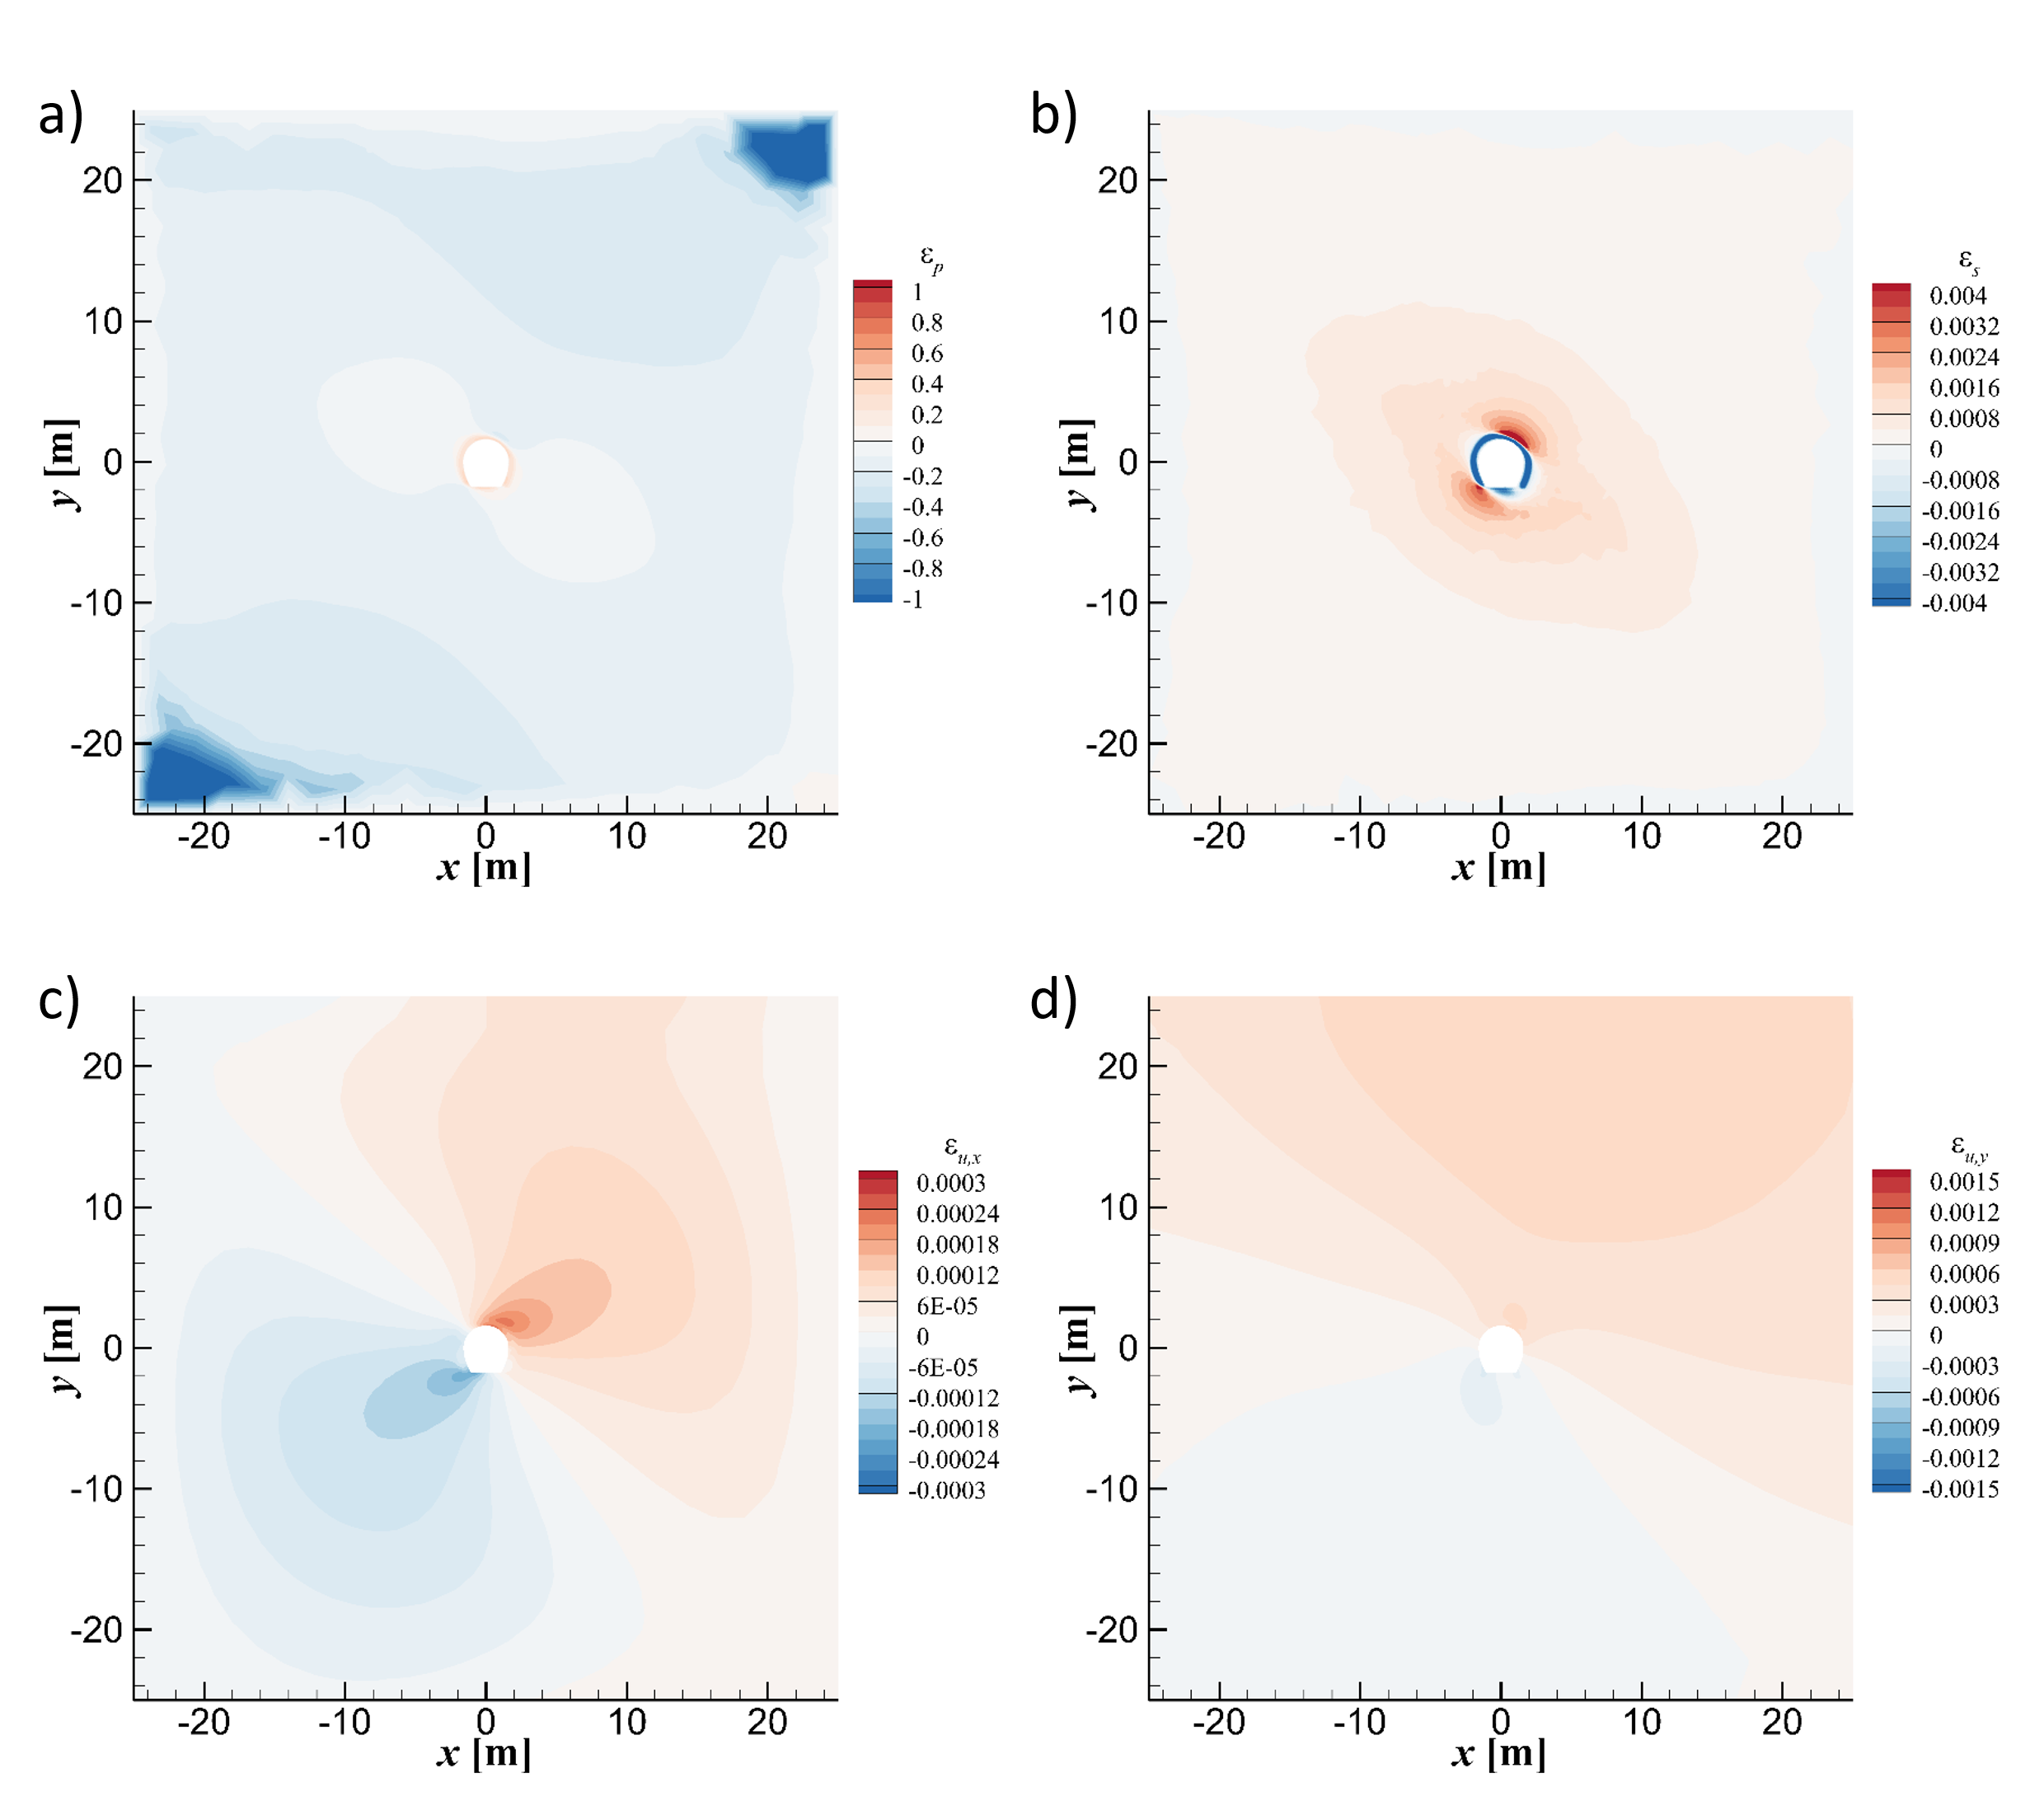
\includegraphics[width=\textwidth]{./figures/MEX10_RM_error_2d_anisotropic.png}
\caption{Deviations between OGS-5 and OGS-6 for anisotropic conditions after 20 years of simulation time.  a) Fluid pressure, b) effective saturation, c) horizontal deformation and d) vertical deformation.}
\label{fig:RM_error_2d_anisotropic}
\end{figure}

\begin{table}
 \caption{Deviations observed when comparing OGS-5 with OGS-6 for the RM process with anisotropic conditions.\label{tab:error_RM_anisotropic}}
\begin{center}
\begin{tabular}{ l | c | c | c }
 Quantity				& $\min{(\epsilon)}$ 	& $\max{(\epsilon)}$	 & RMSE  \\
 \hline
 $p_f$				 	& -1.8785 				& 0.4051 		& $1.27\cdot 10^{-1}$\\ 
 $S_\text{eff}$ 		& -0.0120 				& 0.0090		& $2.51\cdot 10^{-3}$\\		
 $u_x$					& -0.0002 				& 0.0002		& $9.48\cdot 10^{-5}$\\		 
 $u_y$ 					& -0.0004 				& 0.0006		& $2.36\cdot 10^{-4}$\\	
\end{tabular}
\end{center}
\end{table}

%%%%%%%%%%%%%%%%%%%%%%%%%%%%%%%%%%%%%%%%%%%%%%%%%%%%%%%%%%%%%%%%%%%%%%%%%%%%%%%%%%%%%%%%%
\subsection{Code performance}
%%%%%%%%%%%%%%%%%%%%%%%%%%%%%%%%%%%%%%%%%%%%%%%%%%%%%%%%%%%%%%%%%%%%%%%%%%%%%%%%%%%%%%%%%

To compare the performance of the two simulation codes, we measure the wall-clock time for the different simulations runs, which were carried out on a single core on the local \texttt{B2lx06} and \texttt{OGS02} at the BGR. Both systems are equipped with Intel Xeon E5-2690 processors. The processors on the older cluster \texttt{B2lx06} are the version 2 of this type of processor with a clock frequency of  3.0 GHz, whereas the newer cluster \texttt{OGS02} uses version 3 with a clock frequency of 2.6 GHz. Hence, we expect a similar performance for the two systems. For the analysis that follows, we only consider those simulations with a computational mesh of a total of 5463 nodes and 29,200 time steps for the entire simulation time. 

All runtimes recorded for the simulations presented in Sections \ref{sec:RF} and \ref{sec:RM} are summarized in Table \ref{tab:runtime}. The simulation carried out with OGS-5 in Section \ref{sec:RF} took 10 h and 54 min, whereas OGS-6 needed 1 h and 15 min for the same problem. Hence, the computational time of OGS-6 excels over OGS-5 by a factor of 8.6 for the "Richards Flow" model. While the simulation using "Richards Flow" was completed after 1 h 15 min, the simulation using OGS-5 with the model "Richards Mechanics" (Section \ref{sec:RM_no_M}) took 78 h and 20 min on the local cluster \texttt{B2lx06} at BGR, which is more than 3 days. This could be caused by the increased complexity of including mechanic deformation in the integration scheme (Equations \eqref{eq:linear_momentum}--\eqref{eq:hookes_law}). 

On the other hand, the computation for the setup described in Section \ref{sec:full_RM} took 81 h (isotropic conditions) and 153.5 h (anisotropic conditions) on the (faster  and newer) \texttt{OGS02} cluster, while OGS-6 needed 91.6 h (isotropic conditions) and 113.6 h (anisotropic conditions) on the (slower and older) cluster \texttt{B2lx06} to complete the task. This shows that for the computational time becomes comparable for the codes when the full "Richards Mechanics" process is considered. Nevertheless, the fact that OGS-6 uses a stronger coupling suggests that the newly developed OGS-6 is superior to its predecessor version.  A more rigorous speed test on identical hardware would be desirable to gain full insight into the enhanced capabilities of OGS-6.

\begin{table}
 \caption{Runtime for the different simulations presented in Sections \ref{sec:RF} and \ref{sec:RM}. Both systems are run by the BGR and employ Intel Xeon E5-2690 processors. Cluster \texttt{B2lx06} uses version two  with a clock frequency of 3.0 GHz, wheras cluster \texttt{OGS02} uses version 3 with a clock frequency of 2.6 GHz. \label{tab:runtime}}
\begin{center}
\begin{tabular}{ l | r | r | r  }
 Analysis		&  Software & System & Runtime [h]\\ 
 \hline
 \multirow{2}{*}{Section \ref{sec:RF}} 	& OGS-5 & \texttt{OGS02} & 10.9\\
 									& OGS-6 & \texttt{OGS02} &  1.25\\
 \hline 										
 Section \ref{sec:RM_no_M}	& OGS-6 & \texttt{B2lx06} & 78.3\\
 \hline
 \multirow{2}{*}{Section \ref{sec:full_RM} - isotropic} & OGS-5 & \texttt{OGS02} & 81\\
& OGS-6 & \texttt{B2lx06} & 91.6 \\
 \hline
 \multirow{2}{*}{Section  \ref{sec:full_RM} - anisotropic}  & OGS-5 & \texttt{OGS02} & 153.5\\
& OGS-6 & \texttt{B2lx06} & 113.6 \\
\end{tabular}
\end{center}
\end{table}

%%%%%%%%%%%%%%%%%%%%%%%%%%%%%%%%%%%%%%%%%%%%%%%%%%%%%%%%%%%%%%%%%%%%%%%%%%%%%%%%%%%%%%%%%
\subsection{Conclusions}
%%%%%%%%%%%%%%%%%%%%%%%%%%%%%%%%%%%%%%%%%%%%%%%%%%%%%%%%%%%%%%%%%%%%%%%%%%%%%%%%%%%%%%%%%

We have conducted a detailed investigation of a characteristic coupled hydro-mechanical problem of a saturating/desaturating niche in an rock laboratory to compare the accuracy of the newly developed FE-code OGS-6 to its predecessor version OGS-5. We employed characteristic properties of clayrock and apply realistic boundary conditions such as the seasonal change of air humidity  at the wall of the niche and the tranverse isotropic behavior introduced by the bedding of the clayrock in a certain angle of inclination. The aim was to reproduce the results by \cite{ziefle2018}, who successfully computed the hydro-mechanical behavior of a niche in the Mont Terri Rock Laboratory. We built the tests  with increasing complexity starting from uncoupled hydraulic effects to transverse isotropic conditions of the fully coupled hydro-mechanical process. 

As desired, we have found a high degree of agreement between the two codes for the uncoupled hydraulic process "Richards Flow". However, we found differences in the fully hydro-mechanically coupled problem "Richards Mechanics" which may be due to the different coupling schemes employed in the different codes. Further research will be needed to clarify this issue. The new code OGS-6 shows a good performance in terms of wall clock time needed to complete the simulation tasks, although more rigorous testing would be needed to get a better picture of the performance on different systems under controlled operation conditions. Furthermore, the implementation of the governing equations in OGS-6 was found to be of first order in time. The order of convergence in space was found to be 1.6. OGS-6 provides enhanced capabilities for the coupling of the two processes, such as the strongly coupled monolithic scheme that, in general, is more accurate than the weakly coupled staggered scheme. These developments provide a promising starting point for further simulations that allow for high fidelity investigations of coupled processes in clayrock.
